\documentclass[11pt,letterpaper]{article}

% Compile with: xelatex main.tex; bibtex main; xelatex main.tex; xelatex main.tex
% xelatex natively understands UTF-8, no inputenc needed.

\usepackage[margin=1in]{geometry}
\usepackage{fontspec}            % xelatex font selection
\usepackage{amsmath,amssymb,amsthm}
\usepackage{graphicx}
\usepackage{float}
\usepackage{xcolor}
\usepackage{hyperref}
\usepackage[numbers,sort&compress]{natbib}
\usepackage{booktabs}
\usepackage{caption}
\usepackage{longtable}
\usepackage{array}
\usepackage{calc}
% pandoc emits \real{0.2} etc. inside table column specs; provide it.
\providecommand{\real}[1]{#1}
\providecommand{\tightlist}{\setlength{\itemsep}{0pt}\setlength{\parskip}{0pt}}
% pandoc emits \def\LTcaptype{none} to suppress table captions; define the
% counter so longtable doesn't error.
\newcounter{none}
\usepackage{microtype}
\usepackage{titlesec}
\usepackage{newunicodechar}
\usepackage{url}
% Allow line-breaks inside \url{} / \path{} at slashes, underscores,
% dots, hyphens. Output keeps typewriter font.
\PassOptionsToPackage{hyphens}{url}
% No stretchy spacing at break points — keeps path characters tight when
% the line is justified. Breaks are still enabled by \UrlBreaks below.
\Urlmuskip=0mu\relax
% Add break-points after / _ . - so file paths split cleanly.
\renewcommand{\UrlBreaks}{\do\/\do\_\do\.\do\-\do\&\do\?\do\=\do\,\do\;}
% Loosen TeX's line-breaking globally, to absorb any remaining overflow.
\sloppy
\setlength{\emergencystretch}{3em}

% Unicode -> math/text mappings (so utf8 source compiles with pdflatex)
% Greek letters
\newunicodechar{ρ}{\ensuremath{\rho}}
\newunicodechar{μ}{\ensuremath{\mu}}
\newunicodechar{σ}{\ensuremath{\sigma}}
\newunicodechar{ξ}{\ensuremath{\xi}}
\newunicodechar{α}{\ensuremath{\alpha}}
\newunicodechar{β}{\ensuremath{\beta}}
\newunicodechar{γ}{\ensuremath{\gamma}}
\newunicodechar{η}{\ensuremath{\eta}}
\newunicodechar{δ}{\ensuremath{\delta}}
\newunicodechar{ε}{\ensuremath{\varepsilon}}
\newunicodechar{τ}{\ensuremath{\tau}}
\newunicodechar{π}{\ensuremath{\pi}}
\newunicodechar{Φ}{\ensuremath{\Phi}}
\newunicodechar{Δ}{\ensuremath{\Delta}}
% Math operators / scripts
\newunicodechar{²}{\ensuremath{^{2}}}
\newunicodechar{³}{\ensuremath{^{3}}}
\newunicodechar{⁰}{\ensuremath{^{0}}}
\newunicodechar{¹}{\ensuremath{^{1}}}
\newunicodechar{⁴}{\ensuremath{^{4}}}
\newunicodechar{⁵}{\ensuremath{^{5}}}
\newunicodechar{⁶}{\ensuremath{^{6}}}
\newunicodechar{⁷}{\ensuremath{^{7}}}
\newunicodechar{⁸}{\ensuremath{^{8}}}
\newunicodechar{⁹}{\ensuremath{^{9}}}
\newunicodechar{ⁿ}{\ensuremath{^{n}}}
\newunicodechar{⁻}{\ensuremath{^{-}}}
\newunicodechar{ₑ}{\ensuremath{_{\mathrm{e}}}}
\newunicodechar{ᶜ}{\ensuremath{^{c}}}
\newunicodechar{₀}{\ensuremath{_{0}}}
\newunicodechar{₊}{\ensuremath{_{+}}}
\newunicodechar{₋}{\ensuremath{_{-}}}
\newunicodechar{√}{\ensuremath{\sqrt{\,}}}
\newunicodechar{×}{\ensuremath{\times}}
\newunicodechar{−}{\ensuremath{-}}
\newunicodechar{→}{\ensuremath{\rightarrow}}
\newunicodechar{≤}{\ensuremath{\leq}}
\newunicodechar{≥}{\ensuremath{\geq}}
\newunicodechar{≈}{\ensuremath{\approx}}
\newunicodechar{∈}{\ensuremath{\in}}
\newunicodechar{∞}{\ensuremath{\infty}}
\newunicodechar{·}{\ensuremath{\cdot}}
\newunicodechar{±}{\ensuremath{\pm}}
\newunicodechar{∝}{\ensuremath{\propto}}
\newunicodechar{∧}{\ensuremath{\wedge}}
\newunicodechar{∨}{\ensuremath{\vee}}
\newunicodechar{∑}{\ensuremath{\sum}}
\newunicodechar{≠}{\ensuremath{\neq}}
\newunicodechar{≫}{\ensuremath{\gg}}
\newunicodechar{≪}{\ensuremath{\ll}}
% Subscript Latin letters (used in symbols like h_max, J_eff, c_log)
\newunicodechar{ₐ}{\ensuremath{_{a}}}
\newunicodechar{ₓ}{\ensuremath{_{x}}}
\newunicodechar{ₖ}{\ensuremath{_{k}}}
\newunicodechar{ₘ}{\ensuremath{_{m}}}
\newunicodechar{ₚ}{\ensuremath{_{p}}}
\newunicodechar{ₛ}{\ensuremath{_{s}}}
\newunicodechar{ₜ}{\ensuremath{_{t}}}
\newunicodechar{ⱼ}{\ensuremath{_{j}}}
\newunicodechar{≳}{\ensuremath{\gtrsim}}
\newunicodechar{≲}{\ensuremath{\lesssim}}
\newunicodechar{⌊}{\ensuremath{\lfloor}}
\newunicodechar{⌋}{\ensuremath{\rfloor}}
\newunicodechar{⟨}{\ensuremath{\langle}}
\newunicodechar{⟩}{\ensuremath{\rangle}}
\newunicodechar{ℓ}{\ensuremath{\ell}}
% Punctuation
\newunicodechar{§}{\S{}}
\newunicodechar{°}{\textdegree}
\newunicodechar{…}{\ldots}
% Phonetic / IPA / specialty (best-effort fallbacks)
\newunicodechar{ˡ}{\ensuremath{^{l}}}
\newunicodechar{ˣ}{\ensuremath{^{x}}}
\newunicodechar{̄}{}
\newunicodechar{ᐟ}{}
\newunicodechar{ᴅ}{D}
\newunicodechar{ᵒ}{\ensuremath{^{o}}}
\newunicodechar{ᵢ}{\ensuremath{_{i}}}
\newunicodechar{ᵦ}{\ensuremath{_{\beta}}}
\newunicodechar{ő}{\H{o}}
% Additional glyph mappings: glyphs present in the manuscript that had no
% mapping above. Greek set in math mode -> italic for single-letter
% variables (uniform with the mapped ξ, μ, η above).
\newunicodechar{λ}{\ensuremath{\lambda}}
\newunicodechar{ζ}{\ensuremath{\zeta}}
\newunicodechar{φ}{\ensuremath{\varphi}}
\newunicodechar{½}{\ensuremath{\tfrac{1}{2}}}
\newunicodechar{Ẇ}{\ensuremath{\dot{W}}}
\newunicodechar{′}{\ensuremath{{}^\prime}}
\newunicodechar{₂}{\ensuremath{_{2}}}
\newunicodechar{ℤ}{\ensuremath{\mathbb{Z}}}
\newunicodechar{↔}{\ensuremath{\leftrightarrow}}
\newunicodechar{⇒}{\ensuremath{\Rightarrow}}
\newunicodechar{𝒩}{\ensuremath{\mathcal{N}}}

\hypersetup{
  colorlinks=true,
  linkcolor=blue!50!black,
  citecolor=blue!50!black,
  urlcolor=blue!50!black,
}

\titleformat*{\section}{\Large\bfseries}
\titleformat*{\subsection}{\large\bfseries}
\titleformat*{\subsubsection}{\normalsize\bfseries\itshape}

\setlength{\parskip}{4pt}
\setlength{\parindent}{0pt}

\title{Transient Branch Selection and Delivered Stabilizer Amplitude in a Bistable Mean-Field Model:\\
Matched-Seed Measurements of Collapse Probability}
\author{Chowon Jung\\
Department of Computer Science, University of Colorado Boulder, Boulder, Colorado, USA\\
\small\texttt{dancing4am@gmail.com}}
\date{\today}

\usepackage{lineno}
\begin{document}
\linenumbers
\maketitle

\section{Abstract}\label{abstract}

We study a Curie--Weiss stochastic differential equation for an order parameter \emph{m} under coupling \emph{J}, tied to a slow wealth variable \emph{W}(\emph{t}) feeding a protective field \emph{h}(\emph{W}) = 2·(\emph{W}/500). Under matched seeds we measure post-transient wrong-branch selection and wealth collapse (\emph{W} below subsistence); they dissociate under a purely linear consumption rule, the wealth observable a conservative proxy. Collapse proceeds by two channels: an early channel, transient branch selection near the unstable state, described by a parameter-free selection formula (baseline prediction 0.80--1.48× over \emph{J} ≥ 3.5), and a late channel strengthening under a boundary-preserving integrator, its weight open. On the in-domain \emph{h} = 2.4 field the formula under-predicts collapse 5--140× (\emph{J} = 10--20; far more at \emph{J} = 7), unexplained. A pre-registered matched-seed control (weakened stabilizer, α = 0.05) refutes the full-trajectory delivered mean as a predictor: matched-mean fields give 0.281 versus 0.000 (headline cell), REFUTED in all three cells. The coefficient required to hold P(collapse) fixed grows superlinearly in \emph{J} (log--log exponents 1.90--3.62); a theory surface reproduces it for \emph{J} ≥ 3.5 to typically 10--20\% (median 12\%; \emph{R}² = 0.906). The residual approaches one-half as \emph{J} → ∞ under instantaneous onset, a closed-form limit beyond the simulated range.

\section{Keywords}\label{keywords}

mean-field bistability; Curie--Weiss model; stochastic differential equations; noise-induced transitions; common-mode noise; branch selection

\section{Introduction}\label{introduction}

Coupled bistable systems exhibit a generic tension between a coupling favoring synchronized states and a protective bias favoring one of them. We study the simplest stochastic system with both: a Curie--Weiss (mean-field) order parameter \emph{m}(\emph{t}) ∈ (−1, 1) under coupling \emph{J}, subject to multiplicative noise, together with a slow wealth variable \emph{W}(\emph{t}) that feeds an endogenous protective field \emph{h}(\emph{W}) = 2·(\emph{W}/500) tilting the dynamics toward the protective (+\emph{m}) branch (equations (1) and (2), Results). The field is wealth-fed: its magnitude follows current wealth through a fixed conversion rule, not the coupling or the state.

Three measurement questions organize the paper. First, \emph{what is measured}: two observables under matched seeds --- wrong-branch selection after the initial transient and wealth collapse, first passage of \emph{W} below a subsistence threshold; the two dissociate under a purely linear consumption rule (Results), making the wealth observable a conservative proxy for the branch-selection event. Second, \emph{through which channels collapse operates}: an early channel of noise-driven branch selection near the unstable state (Suzuki-type transient selection \cite{suzuki1977} with a parameter-free selection formula; Supplementary Section S2.7) and a late channel of collapses long after the transient --- noise-activated escape from the metastable well, a distinct process the formula under-predicts --- its weight left open. Third, \emph{what decides outcomes in static sweeps} --- we compare the wealth-fed baseline, fixed fields \emph{h} = 2.4 and 5.0, and three response-form variants, with constant-field controls matched to delivered means, plus an inversion of the collapse profile for the required coefficient \(h_0^*(J)\) (Results; Supplementary Sections S5.4 and S5.8).

The mean-field structure of equation (1) has a formal antecedent in the economics of discrete choice: Brock and Durlauf derive the same Curie--Weiss mean-field equation as the equilibrium of a binary-choice model with social interactions \cite{brockdurlauf2001,blume1993}, and the same imperfection-sensitive structure underlies collective opinion shifts \cite{michardbouchaud2005}; equation (1) is a stochastic-dynamical instance with the field endogenized through wealth.

The closest prior work on the dynamics is the stabilized bistable mean-field diffusion of Garnier, Papanicolaou \& Yang \cite{garnier2013}, who show via large deviations that stronger coupling raises the probability of a large collective transition --- the direction we find, reached here by a free-energy-barrier and transient-selection route. We claim no priority for that result: this paper is an application and synthesis adding the two-observable measurement, the delivered-amplitude controls, and the measured superlinear amplitude requirement --- none formulated by Garnier et al.~The cusp catastrophe with a linear imperfection field is the long-established normal form behind the geometry \cite{postonstewart1978}; a discrete-lattice analogue is the critical field for front propagation in coupled cells \cite{kladko2000}.

Adjacent recent measurements --- kinetic-Ising barrier crossing at fixed coupling \cite{oliverbonafoux2026}, a McKean--Vlasov double-well threshold study \cite{abreufilho2025}, an applied Ising enforcement field \cite{zaklan2009}, and the coordination-failure lineage \cite{diamond1982,cooperjohn1988} --- differ in what is measured (comparison, S8 Note 1). Ishii \& Kori \cite{ishiikori2025} classify coupling-regime-dependent mechanisms of noise-induced escape in diffusively coupled bistable ensembles, without a bias field, a selection observable, or a control-amplitude question. Ma et al.~\cite{ma2025feedback} study a feedback Ising model whose coupling depends on the magnetization; here feedback enters through the field \emph{h}(\emph{W}) via a slow variable, and the measurands are selection and collapse probabilities, not equilibrium bifurcations.

Our contribution is threefold; all three are measurement statements. \emph{First}, two observables and two channels: the observables dissociate under a purely linear consumption rule, so wealth collapse is a conservative proxy, and collapse operates through an early channel --- transient branch selection near the unstable state, for which a parameter-free formula reproduces the measured required-amplitude surface in its stated domain (\emph{J} ≥ 3.5), typically to 10--20\% --- and a late channel the formula under-predicts --- a distinct process, noise-activated escape from the metastable well, its weight open (Results; Supplementary Section S9).

\emph{Second}, a pre-registered magnitude-matched control on this paper's matched-seed contrast (Methods): matching a stabilizer's full-trajectory delivered mean does not reproduce its collapse outcome. Two seed-matched fields carrying the same full-trajectory delivered mean give opposite outcomes (P = 0.281 vs 0.000), the verdict REFUTED in all three cells against a decision rule fixed in advance (Results; §S5.6). Whether any single delivered-amplitude summary orders the parameterizations is a domain-dependent exploratory question (§S5.6), not advanced as a contribution.

\emph{Third}, an amplitude requirement with a parameter-free overlay: the wealth-coupling coefficient \(h_0^*(J)\) required to hold P(\emph{W}-collapse) at a fixed target grows superlinearly in \emph{J}; a theory-derived surface reproduces the measurement in its stated domain but misses the near-onset steepening, and the fitted onset sits above the theoretical one by an unexplained offset (Results; Supplementary Sections S5.4 and S5.8).

In sum, this paper claims --- and measures by direct simulation in the specified model --- that collapse proceeds by an early branch-selection channel quantitatively described, in its stated domain (bar an in-domain exception at fixed \emph{h} = 2.4), by a parameter-free selection formula and a late channel identified as noise-activated escape, its weight open; that the two observables measured dissociate under a purely linear consumption rule; that a pre-registered matched-seed control refutes the full-trajectory delivered mean as a predictor of a stabilizer's outcome (0.281 vs 0.000 at the headline cell, REFUTED in all three cells); and that the wealth-coupling coefficient \(h_0^*(J)\) required to hold collapse probability fixed grows superlinearly in the coupling with a fitted onset above the theoretical value. Separately, the one-half residual ceiling is a closed-form property of the selection CDF --- not a simulated measurement --- approached only under instantaneous onset far beyond the simulated range (§S2.7).

All transient-selection and stochastic-escape results are claimed in the common-mode regime (aggregate O(1) order-parameter fluctuations); an \emph{N}-agent extension states this scope, and ramp experiments cover time-dependent coupling (Results; Supplementary Section S6). A cusp/fold + reversibility criterion, probed with two out-of-scope substrates (a third literature-classified) and one confirming corner case, delimits where the picture applies (Discussion).

\section{Results}\label{results}

\subsection{\texorpdfstring{The minimal model, the \emph{h}/\emph{J} scaling, and the two observables}{The minimal model, the h/J scaling, and the two observables}}\label{the-minimal-model-the-hj-scaling-and-the-two-observables}

Let \emph{m}(\emph{t}) ∈ (−1, 1) be the mean-field coordination order parameter and \emph{W}(\emph{t}) the wealth; the minimal model is


\begin{equation*}
\dot m = -m + \tanh\!\left(\frac{J\,m + h(W)}{T}\right) + \xi\,\sqrt{1-m^2}\,\eta(t), \tag{1}
\end{equation*}



\begin{equation*}
\dot W = \mu \cdot \mathrm{employment}(m) - \mathrm{consumption}(W), \tag{2}
\end{equation*}


with employment, consumption, the passive stabilizer field, all fixed parameters, and the sweep ranges of \emph{J} and \emph{μ} as specified in Methods.

The passive/active labeling is a device only (Definition 1, Methods): the controls show that the passive/active label does not by itself carry static-sweep outcomes.

\textbf{Proposition 1} (\emph{h}/\emph{J} \emph{scaling of the tilt-to-barrier ratio}). \emph{In the deterministic mean-field description of equations (1) and (2), the dimensionless ratio η of the field-induced energy asymmetry between the protective (+m) and unprotective (−m) branches to the barrier separating them scales as h/J for J ≫ T, hence decays as 1/J at high coupling.}

\textbf{Two observables.} All measurements report one or both of two \emph{matched-seed} observables (Methods): \emph{wrong-branch selection} and \emph{wealth collapse}, P(\emph{W}-collapse).

P(\emph{W}-collapse)'s visibility depends on the fixed subsistence term of equation (2): under the purely linear consumption rule (Methods) it is 0.000 for \emph{J} ≤ 4.0 at \emph{μ} = 100 (\emph{n} = 2,000; 95\% upper bound 0.0015) and only 0.0865 at \emph{J} = 5.0, while wrong-branch selection reaches 0.2355 --- the same order as under the affine baseline (per-\emph{J} values, Supplementary Section S5.7). This wrong-branch pathology persists under the linear rule at the affine order of magnitude --- suppressed but not eliminated --- while its wealth signature is suppressed; in the affine cells the two observables track the same event (surviving-run P(\emph{m} \textless{} 0 at \emph{t} = 50) ≤ 0.0011).

Proposition 1 concerns the potential's geometry; what it implies for collapse probabilities at finite coupling is an empirical question (Supplementary Section S2.4). The linearization analysis predicts a typing: residual collapses should be \emph{rigidity-typed} (\textbar{}\emph{m}\textbar{} near 1), not \emph{fragmentation-typed} (\textbar{}\emph{m}\textbar{} near 0) (Supplementary Section S2.7).

Measured with the full-grid sweep (Figure 1; Methods): at \emph{J} = 0.5, raising \emph{μ} from 20 to 100 removes collapse (P 1.00 → 0.00); in the band \emph{J} ≥ 4.0 it only reduces P(collapse) from 1.00 to 0.23 --- a persistent residual, 90\% rigidity-typed under clipped Euler--Maruyama (EM) integration (Methods), as predicted. The typing split at the \textbar{}\emph{m}\textbar{} = 0.9 gate is scheme-sensitive and additive noise shifts it toward fragmentation; P(collapse) and timing are robust (Supplementary Sections S4, S5.1; S8 Note 6). Fragmentation occupies the low-\emph{J}, low-\emph{μ} corner; rigidity dominates the high-\emph{J} band at every \emph{μ}. The residual persists because the transient field pins the selection bias \emph{c} while the origin-instability rate \emph{λ} grows with \emph{J}, driving P toward the ½ ceiling (Supplementary Section S2.7); its rigidity typing is the signature of multiplicative noise.

\subsection{The early channel: transient branch selection near the unstable state}\label{the-early-channel-transient-branch-selection-near-the-unstable-state}

At zero noise the drift carries the system from the disordered start onto the protective branch (the positive bias \emph{c}, Supplementary Section S2.7), so the residual is a noise-driven \emph{selection} effect, not a deterministic defect --- Suzuki's transient selection at an unstable state \cite{suzuki1977,tarliemckane1998,mckanetarlie2001,mckanetarlie2004}. Linearizing at the origin gives a parameter-free wrong-branch probability, \(P = \Phi\!\left(-(c/\xi)\sqrt{2/\lambda}\right)\), with \emph{c} and λ evaluated at the effective field \(h_{\mathrm{eff}}\) --- the field during the selection transient (mapping, Methods): ≈0.4 for the wealth-fed baseline, the constant value for fixed fields. The formula saturates toward a ½ ceiling as \emph{J} → ∞ (instantaneous onset from \emph{m} = 0; §S2.7) with no clean power-law exponent: the local log--log slope sweeps from 6.4 to 0.10, passing ≈0.73 near \emph{J} ≈ 4 --- explaining why a pre-specified exponent fit (Methods) found no single exponent (Supplementary Section S2.7).

The formula was checked cell-by-cell (Supplementary Section S5.8). For the wealth-fed baseline (the formula's convention, Methods), predictions lie within a factor of 0.80--2.13 of measurement across \emph{J} = 2.5--10 (mean absolute error 0.054 at \emph{n} = 100/cell, Supplementary Section S5.8). The failures are findings, not fitting problems: the formula under-predicts the \emph{h} = 2.4 failures at \emph{J} = 10, 15, 20 by factors of 140, 12, and 5, and for the fixed \emph{h} = 5.0 cells (\emph{J} = 15, 20) the linearized origin is \emph{stable} (λ ≤ 0): it predicts exactly zero against measured 0.05 and 0.12 (\emph{n} = 100; the paired \emph{n} = 2,000 comparison, where the boundary-preserving scheme runs larger than clipped EM, is in Supplementary Section S4), with the coupling residual cells (also λ ≤ 0) at ≤ 0.01 --- zero-predicted failures that signal a second channel (``The late channel''). The formula is an origin linearization for a static tilted double well and does not apply to the state-dependent stress field (Supplementary Section S5.8); the quadratic variant's residual, by contrast, is predicted to within a factor of 0.92--1.46 from its selection-transient delivered field alone.

\subsection{Delivered-amplitude controls: what the static contrasts measure}\label{delivered-amplitude-controls-what-the-static-contrasts-measure}

The \emph{delivered} field and \emph{delivered mean} are defined in Methods. We replaced the wealth-fed base field with a stress, a coupling, and a quadratic variant (forms and coefficient α, Methods) in the same matched-seed full-grid sweep, pre-specified. At α = 2.0 (stress) / α = 1.0 (coupling) the baseline high-\emph{J} residual (0.23 band-averaged at \emph{μ} = 100; single-cell 0.28--0.41, Supplementary Section S4 and the Supplementary Section S5.2 one-at-a-time baseline, an independent seed set, for the 0.41) is absent: P(collapse) = 0.00 across \emph{J} ≥ 4.0 at \emph{μ} = 100 for the stress form and ≤ 0.01 for the coupling form (Figure 2; bounds, S8 Note 3). The quadratic form retains a band-mean residual of 0.14 at α = 1.0 (0.13, 0.11, 0.17 at \emph{J} = 4.0, 4.5, 5.0; Supplementary Sections S5.1, S8 Note 3).

The pre-specified contrast stands as a measurement; its \emph{interpretation} is revised by three controls (Supplementary Section S5.6); we state the revision openly as this version's correction. First, \emph{J} is constant within every static-sweep run, so the coupling and quadratic forms are per-\emph{J} constant \emph{rescalings} of the base field --- definitionally a delivered-magnitude comparison (equilibrium values, S8 Note 3). Second, a pre-registered magnitude-matched control shows that matching a stabilizer's full-trajectory delivered mean does not reproduce its collapse outcome. At the informative operating point (α = 0.05) the stress form and a pure constant carrying the same full-trajectory delivered mean (≈11.7) give opposite collapse probabilities --- 0.281 versus 0.000 at the headline cell --- the pre-specified verdict REFUTED in all three cells (paired difference 0.234--0.281, all 95\% CIs excluding 0; Supplementary Section S5.6). The large constant over-protects the early selection transient (Supplementary Section S5.6). Whether any single delivered-amplitude summary orders the parameterizations is examined in Supplementary Section S5.6 as an exploratory measurement; the ordering breaks only through the state-dependent stress arm that the formula's domain rule excludes, so we do not advance it as a result. Third, among the \emph{constant} fields a low delivered amplitude tracks collapse: the wealth-fed baseline delivers only ≈0.4 when the branch is selected (Methods) and fails, whereas the fixed fields 2.4 and 5.0 hold P(\emph{W}-collapse) ≤ 0.001 in the calibrated range (\emph{J} = 3 and 5, \emph{μ} = 100).

Beyond the calibrated range the fixed fields begin to fail: their tilt-to-barrier ratio \emph{η} (Methods) shrinks as \emph{J} grows --- the \emph{h} = 2.4 field fails from \emph{J} ≈ 7 and the \emph{h} = 5.0 field later, reaching P(\emph{W}-collapse) ≈ 0.08--0.27 by \emph{J} = 20 while remaining below the wealth-fed baseline at every \emph{J} (clipped-EM, \emph{n} = 1,000; d\emph{t}-converged under both integrators; Supplementary Sections S5.1, S4, S8 Note 3), while the coupling form's rescaled field stays at P ≤ 0.02 (\emph{n} = 100; \texttt{scaling\_control.csv}); whether the \emph{η}-decay sets their onset is open (Supplementary Section S5.8). These \emph{J} = 7--20 points probe the small-\emph{η} regime.

\subsection{\texorpdfstring{The amplitude requirement \(h_0^*(J)\) and a parameter-free overlay}{The amplitude requirement h\_0\^{}*(J) and a parameter-free overlay}}\label{the-amplitude-requirement-h_0j-and-a-parameter-free-overlay}

A complementary measurement inverts the matched-seed profile P(collapse \textbar{} \emph{h}₀) (grid and protocol, Methods; Supplementary Section S5.4). The required amplitude \(h_0^*(J)\) grows superlinearly: the fitted exponent \emph{p} (log--log fit, Methods) spans 1.90--3.62, with \emph{p} = 1 excluded by the 95\% bootstrap CI in all nine (\emph{ξ}, target) conditions, varying systematically with target and noise. A three-parameter description \(h_0^* = A\,(J - J_{\mathrm{c}})^{p'}\) fits better (\emph{R}² ≥ 0.986, exponent \emph{p}′ = 0.52--1.23); \(J_{\mathrm{c}}\) is a \emph{fitted} quantity (2.16--2.44), not the deterministic bifurcation point \emph{J} = \emph{T} = 2 --- the free fits reject \(J_{\mathrm{c}}\) = 2 in six of eight comparable conditions, and a descriptor pinning the onset at 2 is not adopted (Supplementary Sections S5.4, S8 Note 4). Both descriptions are local to 2.5 ≤ \emph{J} ≤ 5.0, \emph{μ} = 100.

The selection formula of Supplementary Section S2.7 predicts this surface with no fitted parameters: solved for the required field and mapped through the selection-transient wealth (Supplementary Section S5.8), the theory reproduces the measured surface in its stated domain \emph{J} ≥ 3.5 typically to 10--20\% (median 12\%, \emph{R}² = 0.906), though not to within the tight \emph{n} = 2,000 CIs. It does not reproduce the near-onset steepening (over-predicting \(h_0^*\) by up to a factor of 6 at \emph{J} \textless{} 3.5), the in-domain log--log slope, or the onset itself --- the theory's \(h_0^*\) → 0 point sits at \emph{J} = 2.00 exactly, below every unflagged fitted \(J_{\mathrm{c}}\) (2.16--2.44) by 7--18\%; the offset has the expected sign but no quantitative account, and is left open (slope values, Supplementary Section S8, Note 4).

\subsection{The late channel: collapses long after the transient}\label{the-late-channel-collapses-long-after-the-transient}

Collapse timing separates the two channels (Supplementary Section S5.7). The wealth-fed baseline's residual is purely early-transient: at \emph{μ} = 100 every collapse occurs by \emph{t} = 42, and the fraction after \emph{t} = 100 is exactly zero. The fixed-field failures beyond the calibrated range are a \emph{mixture}: median collapse times are passive-like, sharing the selection channel's early timing, but 8--28\% occur after \emph{t} = 100 (99th percentiles ≈779--985; clipped-EM, \emph{n} = 1,000; §S5.7) --- a late channel with zero counterpart in the baseline.

The late channel is not a clipping artifact: under a boundary-preserving scheme (Methods) with paired noise (\emph{n} = 2,000 per cell) it survives and strengthens (Supplementary Sections S4, S9).

Two of three pre-registered tests (Supplementary Section S9) support identifying this channel as noise-activated (Kramers) escape from the metastable well: starting deep in the protected well removes 96.6\% of early collapses while leaving the late-escape rate unchanged (per-cell ratios 0.97--1.13, cells meeting the pre-specified rule of ≥ 10 late events per arm), and the late rate is Arrhenius in the deterministic barrier (\emph{R}² = 0.95; ξ-consistency slope on the effective barrier within the pre-declared band). The third pre-registered test --- waiting-time memorylessness --- failed its coefficient-of-variation / Kolmogorov--Smirnov (CV/KS) threshold, in the direction expected from right-truncation by the finite observation window (Supplementary Section S9.3). A further consistency check, not pre-registered: the monostable (\emph{h} = 5.0, \emph{J} = 7) cell, with no barrier to cross, gives exactly zero late collapses. Under the pre-declared overall rule the identification is supported. The λ ≤ 0 cells (\emph{h} = 5.0 at \emph{J} = 15, 20), where the formula predicts zero, mix the two channels: most collapses are early (77--85\% by \emph{t} = 100; clipped-EM, \emph{n} = 1,000, Supplementary Section S5.7), the early component vanishes under deep-well starts, and the late remainder carries the escape channel's initial-condition-independent hazard (scheme dependence of the early/late split, Supplementary Section S9). Both components lie outside the origin-linearized formula's domain (\emph{λ} ≤ 0), so its failure on these \emph{h} = 5.0 cells is expected; the in-domain \emph{h} = 2.4 under-prediction (above; §S5.8) is a separate, unexplained finding. The weight at the highest couplings remains open: P(collapse) is d\emph{t}-converged, the \emph{J} = 20 late-fraction share is not (§S4).

\subsection{Ramp experiments: where rate and response effects operate}\label{ramp-experiments-where-rate-and-response-effects-operate}

Genuine rate-of-onset effects appear only when the coupling varies, via a schedule \emph{J}(\emph{t}): \emph{gradual}, \emph{exponential}, or \emph{sudden} (forms, Methods) --- the last the instantaneous-onset conditioning of the ½ selection ceiling. Across the three schedules (Methods), gradual and exponential survive at every margin \emph{μ} ≥ 60 (P(collapse) ≤ 0.04), whereas sudden onset triggers rigidity collapse at the lower margins (\emph{μ} ≤ 90; up to 0.47 at \emph{μ} = 40; rigidity ≥ 77\% of collapsed runs at margins with \emph{n} ≥ 10 collapses, clipped-EM gate; per-margin values, S8 Note 5).

A ramp-duration sweep (Figure 3; Methods) shows three regimes: \emph{resilient} (\emph{μ} ≥ 60, P ≤ 0.07); \emph{critical} (\emph{μ} = 50, P rising from 0.19 to a ≈0.50 plateau, 0.50 near 9,200 steps; profile, S8 Note 5); \emph{unviable} (\emph{μ} = 40: P saturates at 1.00 by ramp ≈4,000 steps). Slow ramps remove collapse at high margins, but near the viability margin the ramp does not delay collapse: at \emph{μ} = 40 the median collapse time is ≈21 time units regardless of ramp duration, so under long ramps collapse occurs while the coupling is still near its starting value (the median coupling at collapse, ≈0.56 for the 30,000-step ramp, is the schedule read at that early time, not a ramp effect), and the cell matches the static (\emph{J} = 0.5, \emph{μ} = 40) cell (P = 1.00), with fragmentation the largest typed class (≈0.54 at \emph{μ} = 40, the rest mixed; clipped-EM \textbar{}\emph{m}\textbar{} \textless{} 0.3 gate, Supplementary Section S4), consistent with Figure 1's low-\emph{J}, low-\emph{μ} corner. What triggers these early low-coupling collapses is left open; below the margin, no tested ramp speed avoids collapse.

\subsection{Robustness: ablation cascade, boundary and definition integrity, and reduction validity}\label{robustness-ablation-cascade-boundary-and-definition-integrity-and-reduction-validity}

\textbf{Ablation cascade} (Methods; Supplementary Sections S1 and S5). \textbf{Level 0} (bare SDE, fixed \emph{h}) reproduces the ordered branch with residual selection at high \emph{J} (Supplementary Figure S1). \textbf{Level 1} (minimal model): residual \textbf{23\%} at \emph{μ} = 100, 90\% rigidity. \textbf{Level 2} (belief dynamics; Methods, S1): residual \textbf{30\%}, rigidity 83\%. \textbf{Level 3} (Minsky--Keen credit cycles): residual \textbf{34\%}, rigidity 81\%. The residual's point estimates increase (Figure 4): L1 → L3 +0.11 (unpaired 95\% CI {[}+0.04, +0.18{]}), adjacent steps within sampling error; rigidity dominance preserved (clipped-EM gate, Supplementary Section S4); \textbf{Level 4} (full simulator, d\emph{t} = 0.1) reports a 30--35\% rigidity-dominated band consistent with the L1 → L3 trend (not re-run at d\emph{t} = 0.05; Supplementary Section S1.3). The minimal model is the most optimistic case tested.

\textbf{Orthogonal variations.} A high-\emph{J} sweep (Supplementary Section S5.1, Figure S2) shows that the residual is robust to log-vs-linear \emph{h}(\emph{W}) and substantially \emph{worse} under constant \emph{h} = 0.4; under additive noise at the headline cell (\emph{J} = 5, \emph{μ} = 100) P(collapse) is 0.20 with rigidity share 0.30 (clipped-EM gate; scheme caveat, Supplementary Section S4), so the asymmetry persists but its rigidity signature is noise-prescription-specific (Supplementary Section S5.1). It also holds across voter, Kuramoto, and cubic-Landau variants (Supplementary Section S5.3, Figure S4), within the cusp + reversible scope.

\textbf{Boundary, definition, and horizon integrity.} Clip events are pervasive (≈35\% upper-boundary and ≈2\% lower-boundary trajectory-steps at the headline cell; Supplementary Section S8, Note 6) but the boundaries are non-absorbing (classification, Methods, §S4); a paired boundary-preserving comparison gives P(collapse) 0.307 (clipped-EM) vs 0.295, median collapse step 292 vs 295 (\emph{n} = 2,000) --- probability and timing robust --- while the typing split at the \textbar{}\emph{m}\textbar{} = 0.9 gate is the one scheme-sensitive statistic (0.881 vs 0.744; fragmentation ≤ 0.2\% in both), so type shares carry this scheme caveat (Supplementary Sections S4, S8 Note 6). Collapse-definition perturbations at the headline cell (\emph{J} = 5, \emph{μ} = 100, passive) move P(collapse) only over 0.2985--0.3100 (1.15 pp, \emph{n} = 2,000), gate perturbations move the rigidity share over 0.80--0.95 with fragmentation 0.0000 throughout, and horizon extension to \emph{t} = 4,000 adds no collapses beyond \emph{t} = 250 in the \emph{μ} = 100 baseline cells (§S4, S8 Note 6).

\textbf{Network extension and reduction validity.} An agent-based model (ABM) extension (Methods; Supplementary Section S6) reduces \emph{exactly} to the one-dimensional SDE --- the five uniform-field topologies give bit-identical per-seed outcomes (P(collapse) = 0.33 each at the headline cell, 100 seeds) --- and the one symmetry-breaking variant is not separated from it (0.37 vs 0.33; two-proportion \emph{z} = 0.59, two-sided \emph{P} = 0.55, \emph{n} = 100 seeds per arm). Under purely idiosyncratic noise, order-parameter noise averages as \(\propto 1/\sqrt{N}\) and collapse does not arise at \emph{N} = 200 on any topology; the scalar model at matched \(\sigma_{\mathrm{eff}}\) (formula, Methods) reproduces the ABM statistics within sampling error (largest gap ≈2 SE; Figure 5; Supplementary Sections S6, S8 Note 7) --- the scalar results are claims about common-mode-dominated systems; no network or \emph{N} effect is claimed.

\section{Discussion}\label{discussion}

The central results are three measurements. First, under a purely linear consumption rule the two observables dissociate, so the wealth observable is a conservative proxy, and collapse operates through an early transient-selection channel that a parameter-free formula reproduces in its stated domain --- bar one in-domain exception, the fixed \emph{h} = 2.4 field it under-predicts 5--140× (§S5.8) --- plus a late channel of noise-activated escape from the metastable well, a distinct process whose weight remains open. Second, a pre-registered magnitude-matched control shows that matching a stabilizer's full-trajectory delivered mean does not reproduce its collapse outcome (REFUTED in all three cells); the pre-specified contrast stands as a measurement, and genuine rate-of-onset effects appear only under time-varying coupling. Third, the wealth-coupling coefficient \(h_0^*(J)\) required to hold P(collapse) fixed grows superlinearly in \emph{J}, with a parameter-free overlay that reproduces the surface in-domain but misses the near-onset steepening and the fitted onset (§S5.4, §S5.8). The residual asymmetry and its rigidity typing survive the ablation cascade and four bistable model classes within the common-mode regime.

The results apply within a delimited scope: the predictions follow from a bistable potential that is a \emph{tilted cusp} --- a ℤ₂-symmetric double well with a bounded linear field --- traversed reversibly, whose high-coupling imperfection response is the \emph{h}/\emph{J} decay (Proposition 1; \cite{postonstewart1978}; Supplementary Sections S2.4--S2.6). Fold-type bistability (saddle-node, transcritical; \(\sqrt{h}\) response, privileged equilibrium) is structurally outside, as are glassy non-reversible landscapes; this is a \emph{criterion}, not a theorem --- the cusp/fold clause derives from catastrophe theory, the reversibility clause rests on a heuristic (S8 Note 8). (The coupling sweep is exogenously forced, not self-organized \cite{baktang1987}.) Three substrates lie structurally outside it and do not enter the positive evidence: SIR epidemics (transcritical at \emph{R}₀ = 1; no bistable cells arose in a broad scan) \cite{vandendriessche2002,hadeler1997}; power-grid cascades (saddle-node) \cite{schaefer2018,manik2017,witthaut2022}; and phase-retrieval neural-network training, fold/first-order with hysteresis, where most tested seeds failed adiabatic reversibility \cite{mannelli2019,mondelli2019}. The cusp + reversible corner was completed with the degenerate optical parametric oscillator (DOPO) \cite{drummond1980,drummond1981,wang2013cim,marandi2014}: pre-specified pilot measurements (\protect\path|scope_probes/substrate_D_DOPO/|) confirmed the near-cusp field exponent (excluding the fold value), matched the parameter-free near-threshold coefficient, and passed the adiabatic-reversibility test most neural-network seeds failed (a secondary, confirmatory-only deep-well test was inconclusive; S8 Note 8). DOPO is corner-completion --- a high-confidence confirmation, not a risky falsification test.

Several limitations and open questions remain. The selection and escape results are scoped to common-mode noise --- order parameters carrying aggregate O(1) fluctuations --- not purely idiosyncratic noise at large \emph{N}, where fluctuations are suppressed as \(\propto 1/\sqrt{N}\) and the dynamics become effectively noiseless (Supplementary Section S6); heterogeneous fields, sparser mixed-noise regimes, adaptive rewiring, and strategic feedback remain untested. The delivered-amplitude account rests on a matched-constant control for the stress form (§S5.6), delivered-magnitude comparisons of the coupling and quadratic rescalings, and two fixed fields, not arbitrary response rules. Four quantitative gaps remain: (i) on the in-domain fixed \emph{h} = 2.4 field the formula under-predicts collapse by 5--140× (far more at \emph{J} = 7; §S5.8); (ii) the fitted onset of the amplitude requirement sits above the theory's onset in every unflagged condition, unexplained; (iii) the late channel is noise-activated escape (Supplementary Section S9), a distinct process, but its weight at the highest couplings remains open (not d\emph{t}-converged at \emph{J} = 20; Supplementary Section S4); (iv) collapse-type shares at the \textbar{}\emph{m}\textbar{} = 0.9 gate are integrator-scheme-sensitive (scheme caveat, Supplementary Section S4), while P(collapse) and timing are robust.

Finally, the paper contains no observational-domain applications because a registered shape test failed to confirm the model; we report the deciding measurement for transparency. An earlier stage paired the model with observational analyses, and a pre-registered test compared its \emph{specific} functional shape for event probability against flexible monotone alternatives (protocol, Methods). At the pre-registered 5\%-drawdown threshold the model's simulated-curve encoding was \textbf{disfavored}: ΔOOS = +0.033 nats worse than the best generic monotone alternative. The verdict was encoding-sensitive (a smooth analytical-index encoding of the \emph{same} model was best at all three thresholds, and the two pre-declared secondary thresholds reversed the sign), so we read it as a registered test that fails to confirm the model --- not evidence the model is wrong --- and insufficient support for headline observational claims. The same analyses fixed the honest precision: integrated autocorrelation 60--115 across overlapping windows gave an effective sample of ≈47--90 windows, and all interval estimates used a moving-block bootstrap --- retained as the bar for any future observational application.

Next steps: what governs the crossover between the two channels; an account of the onset offset; endogenous \emph{J}--\emph{W} coupling; a sufficiency proof for the reversibility clause; and further cusp + reversible substrates at the criterion boundary.

\section{Methods}\label{methods}

\subsection{Model specification}\label{model-specification}

The minimal model couples a Curie--Weiss stochastic differential equation in the order parameter \emph{m}(\emph{t}) ∈ (−1, 1) to a deterministic wealth equation \emph{W}(\emph{t}); it is given by equations (1) and (2) of Results, with employment(\emph{m}) = (1 + \emph{m})/2, consumption(\emph{W}) = 30 + 10·(\emph{W}/500), and the passive stabilizer field \emph{h}(\emph{W}) = 2·(\emph{W}/500). We interpret the noise term in the Itô sense throughout. The noise \emph{η}(\emph{t}) in equation (1) is white noise, distinct from Proposition 1's \emph{η}; the selection-transient noise \emph{ζ}(\emph{t}) is defined in Supplementary Section S2.7. The selection formula (Results) uses \(\Phi\), the standard-normal cumulative distribution function, with argument \(-(c/\xi)\sqrt{2/\lambda}\), where \(c = \tanh(h_{\mathrm{eff}}/T)\) and \(\lambda = -1 + (J/T)\operatorname{sech}^2(h_{\mathrm{eff}}/T)\) is the drift-linearization coefficient at the origin (Supplementary Section S2.7); \(\lambda \le 0\) marks a linearly stable origin, outside the formula's domain. The symbol \emph{α} denotes the stabilizer response coefficient defined below; the separately pre-registered ``α-fit'' (\texttt{PREREG\_alpha\_fit\_2026-05-30.md}) is an unrelated fit of the collapse-residual scaling exponent in \emph{J}. Fixed parameters: temperature \emph{T} = 2, noise amplitude \emph{ξ} = 0.5, integration step d\emph{t} = 0.05. Initial conditions \emph{m}(0) = 0, \emph{W}(0) = 100. A clipping rule \emph{m} ∈ {[}−1 + ε, 1 − ε{]} with ε = 10⁻⁶ keeps the multiplicative noise term numerically well-defined at saturation. The multiplicative form \(\sqrt{1-m^2}\) is the canonical prescription for bounded order parameters, compressing fluctuations as the state saturates. By the §S4 Feller criterion each boundary is regular (attainable, reflecting) or entrance (unattainable) depending on (\emph{h}, \emph{J}): the upper boundary is regular wherever \emph{J} + \emph{h} ≳ 1.95 and entrance in the low-coupling, low-field corner; the lower boundary is entrance for \emph{h} ≳ \emph{J} − 1.95 (e.g.~the fixed \emph{h} = 5.0 cell at \emph{J} = 5) and regular otherwise (e.g.~\emph{h} = 5.0 at \emph{J} = 15, 20, where lower-boundary clips are measured). In all cases neither boundary is absorbing (Supplementary Section S4). The clipping rule's residual discretization effect is quantified against a boundary-preserving scheme there; the ε = 10⁻⁶ buffer prevents division-by-zero artifacts without affecting the collapse probability or timing, as confirmed by the Level 0 mean-field validation (Supplementary Figure S1), the convergence check, and the boundary-integrity check (Supplementary Section S4). Wealth is floored at zero each step (\emph{W} ≥ 0, so \emph{h} ≥ 0). At \emph{μ} = 20, maximum income (\emph{μ}·1 = 20) cannot exceed the subsistence constant 30, so collapse is deterministic there. The sweep parameters are the coupling \emph{J} and the income multiplier \emph{μ}, which sets the field's growth rate. The economic terms are mnemonic labels, not empirical claims (Supplementary Section S8, Note 2; Supplementary Section S5.5).

We label \emph{h} the \emph{passive stabilizer} --- restoring force bounded by a constant independent of state and coupling, vs \emph{active}: state-dependent, unbounded under stress (Definition 1, formal statement in Supplementary Section S8, Note 2); the label is a device only.

\subsection{Observables}\label{observables}

All measurements report one or both of two \emph{matched-seed} observables --- within each matched-seed experiment (the stabilizer variants, the magnitude-matched controls, the branch-observable and fixed-field runs) compared conditions reuse identical per-run noise realizations, so those contrasts are paired; the ablation levels use independent seed bases (Supplementary Section S1). The first is \emph{wrong-branch selection}, P(wrong branch at \emph{t} = 50): the fraction of runs with \emph{m} \textless{} 0 at \emph{t} = 50. We call \emph{t} ≤ 50 the \emph{decision window}, and the far shorter O(1) interval just after initialization --- where the branch is selected and the wealth-fed field is still near \emph{h}(\emph{W}₀) ≈ 0.4 --- the \emph{selection transient}. The second is \emph{wealth collapse}, P(\emph{W}-collapse): first passage of \emph{W} below 10 sustained for 200 consecutive steps (10 time units). Wrong-branch selection is read at \emph{t} = 50 --- beyond every observed passive-baseline collapse time (all ≤ 42 at \emph{μ} = 100; Supplementary Section S5.7) yet early in the \emph{t} = 1,000 horizon.

\subsection{Status of the wealth equation}\label{status-of-the-wealth-equation}

Equation (2) is a modeling choice: the affine consumption term 30 + 10·(\emph{W}/500), with wealth floored (clamped) at \emph{W} = 0 at each integration step, is neither derived from first principles nor empirically calibrated. It encodes two qualitative assumptions --- a fixed subsistence cost (the constant 30) and a weakly wealth-dependent component (the slope 10/500) --- and the floor prevents unbounded debt. In herding models of markets the corresponding macro-feedback is conventionally written as price dynamics rather than wealth accumulation \cite{lux1995,contbouchaud2000}; equation (2) differs from that convention. To delimit the range over which the conclusions hold, we repeated the analysis under ±30\% perturbations of both consumption parameters ((21, 10), (39, 10), (30, 7), (30, 13)) and under a structurally different, purely linear consumption rule \emph{C}(\emph{W}) = 0.08·\emph{W} (matched to the baseline total consumption of 40 at \emph{W} = 500, with no subsistence constant); \emph{n} = 2,000 matched-seed paths per cell, 1,000-replicate bootstrap. Under the four parametric perturbations, P(collapse) at the operating point (\emph{h}₀ = 2, \emph{ξ} = 0.5, \emph{μ} = 100) shifts by at most 0.047 in absolute probability over the supercritical range \emph{J} ∈ {[}2.5, 5{]}, the monotone increase of P(collapse) with \emph{J} is preserved, and the amplitude-requirement exponent \emph{p} of Supplementary Section S5.4 (at the P = 0.30 level) stays within {[}2.55, 5.19{]} around the baseline 3.55 --- far from 1 in every parametric variant, so the superlinear amplitude requirement is unchanged. The purely linear rule, by contrast, suppresses wealth collapse almost entirely (P ≤ 0.09 for all \emph{J} ≤ 5, so the P = 0.30 level is unreachable and \emph{p} is undefined) while leaving the branch-selection observable at the same order as the baseline (Results; Supplementary Section S5.7): the fixed subsistence term --- not its precise value, and not the wealth-dependent slope --- is the structural ingredient of equation (2) on which the \emph{wealth-collapse visibility} of the branch pathology depends. Conclusions are therefore robust to ±30\% recalibration of equation (2), and the wealth-collapse observable is conditional on the presence of a fixed subsistence cost (full tables, Supplementary Sections S5.5 and S5.7).

\subsection{Proposition 1 derivation}\label{proposition-1-derivation}

The derivation proceeds from the deterministic fixed-point equation \emph{m} = tanh{[}(\emph{Jm} + \emph{h})/\emph{T}{]}, which has saturated solutions at \emph{m} ≈ ±1 for \emph{J} ≫ \emph{T}. Linearizing each saturated branch yields a branch asymmetry --- the preferential stability of the protective (+m) over the unprotective (−m) branch --- scaling as \emph{h}/\emph{J} to leading order, so it vanishes at high coupling --- and because the field is bounded by equilibrium wealth (itself bounded by \emph{μ}), this holds regardless of how large \emph{μ} is made. We write \emph{η} = \(\Delta{}V_{\mathrm{tilt}}\)/\(\Delta{}V_{\mathrm{barrier}}\) ≈ 4\emph{h}/\emph{J} throughout (barrier ceiling ½ --- distinct from the ½ residual ceiling reported in Results --- and tilt ≈2\emph{h}/\emph{J}); \emph{h} is bounded by equilibrium wealth, so \emph{η} vanishes at high coupling. Full a priori derivation in Supplementary Section S2.

\subsection{Simulation protocols}\label{simulation-protocols}

Runs use an Euler--Maruyama (EM) scheme at d\emph{t} = 0.05 over 20,000 steps (step size fixed by a three-point convergence test --- P(collapse) 0.25 at d\emph{t} = 0.1 vs 0.35 at d\emph{t} ∈ \{0.05, 0.025\}; Supplementary Section S4). The ablation cascade adds complexity one level at a time under the identical sweep and protocol, with an independent seed base per level (Supplementary Sections S1 and S5). The static sweep is \emph{J} ∈ \{0.5, 1.0, \ldots, 5.0\} × \emph{μ} ∈ \{20, 30, \ldots, 100\}, 100 deterministically seeded runs per cell; a run is \emph{collapsed} if \emph{W} \textless{} 10 (1/10 of \emph{W}(0)) for 200 consecutive steps, and \emph{rigidity-} / \emph{fragmentation-typed} if \textbar{}\emph{m}\textbar{} \textgreater{} 0.9 / \textless{} 0.3 at collapse, else \emph{mixed} (the seed formula is given under ``Code availability''; the sweep grid is stated above; the L2--L4 ablation specifications are in Supplementary Section S1). The branch-selection observable is P(\emph{m} \textless{} 0 at \emph{t} = 50) on the same runs. In the Level 2 ablation the field is attenuated as \(h_{\mathrm{eff}}\) = \emph{h}·EC, where EC(\emph{t}) ∈ {[}0, 1{]} is the normalized entropy of the \emph{K} = 6 belief distribution (Supplementary Section S1).

Dynamic-\emph{J} runs replace static \emph{J} with gradual (a linear ramp from \emph{J} = 0.5 to 5.0), exponential (a late-saturating S-curve), and sudden (step) schedules, compared at 100 seeds × 9 \emph{μ} levels × 3 schedules over 30,000 steps at d\emph{t} = 0.05; the ramp-duration sweep runs six ramp durations (1,000--30,000 steps) across nine \emph{μ} levels at 100 seeds per point (5,400 runs; Results, ``Ramp experiments'').

By the \emph{delivered} field we mean the field magnitude realized along a trajectory, \emph{h}(\emph{W}(\emph{t}), \emph{m}(\emph{t})) --- a function of the realized wealth and, for the state-dependent forms, the realized order parameter --- as distinct from the rule's functional form; its time average over a stated interval is the \emph{delivered mean} (Supplementary Section S5.6). The stabilizer-variant experiment reuses the passive SDE, grid, seeds, and collapse criteria under a matched-seed design, replacing \emph{h}(\emph{W}) = 2·(\emph{W}/500) with the stress form \emph{h} = 2·(\emph{W}/500) + α·max(0, −\emph{m})·\emph{J}, the coupling form \emph{h} = 2·(\emph{W}/500)·(1 + α·\emph{J}), or the quadratic form \emph{h} = 2·(\emph{W}/500)·(1 + α·(\emph{J}/5)²) (full-grid runs at α = 2.0, 1.0, and 1.0 respectively; \protect\path|simulation/results/active_stabilizer/active_stress_summary.csv|, \texttt{active\_coupling\_summary.csv}, \texttt{active\_quadratic\_summary.csv}). The α-sweep over all three forms (α ∈ \{0.1, 0.25, 0.5, 1.0, 2.0, 5.0\}, high-\emph{J} band, 100 seeds/cell) is tabulated in Supplementary Section S5.1 (\texttt{alpha\_sweep\_results.csv}); the \emph{J} ∈ {[}6, 10{]} extension of the sweep is archived at \protect\path|simulation/results/extended_sweep/| (reconstruction \texttt{extended\_sweep.py}, statistically consistent --- the original producer predates the deposit, see Data availability; the \emph{J} ≤ 5 grid is in \protect\path|simulation/results/minimal_model/|). The extended-\emph{J} control runs matched-seed sweeps on the coarser grid \emph{J} ∈ \{3, 5, 7, 10, 15, 20\} for the wealth-fed, fixed (\emph{h} = 2.4, 5.0), and coupling fields (Supplementary Section S5.1; \protect\path|simulation/results/active_stabilizer/scaling_control.csv|). The magnitude-matched constant-field controls, the branch-observable and collapse-timing runs (including the linear-consumption dissociation cells), the selection-formula and theory-overlay computations, and the boundary-integrity, late-channel, and collapse-definition checks are specified in Supplementary Sections S5.6, S5.7, S5.8, and S4 respectively. The collapse-definition check perturbs the definition on a 3×3 grid at the headline cell; the horizon-extension check runs three cells (\emph{J} ∈ \{2.5, 3.5, 5.0\} at \emph{μ} = 100) to \emph{t} = 4,000. The theory overlay maps the required field through the selection-transient wealth as \(h_{\mathrm{eff}}\) = 0.2·\emph{h}₀ (derivation, Supplementary Section S5.8). The amplitude-requirement measurement generalizes the passive coefficient to \emph{h}(\emph{W}) = \emph{h}₀·(\emph{W}/500) (baseline \emph{h}₀ = 2) and inverts the matched-seed profile P(collapse \textbar{} \emph{h}₀) on an \emph{h}₀ ∈ {[}0, 6{]} grid; \(h_0^*(J)\) denotes the smallest \emph{h}₀ holding P(collapse) at the stated target. The inversion runs at collapse-probability targets P ∈ \{0.1, 0.2, 0.3\}, over the swept couplings and noise levels, 2,000 paths per (\emph{J}, \emph{ξ}, \emph{h}₀) cell, with 1,000-replicate path-level bootstrap and exponents fitted as log \(h_0^*\) = \emph{a} + \emph{p}·log \emph{J} (Supplementary Section S5.4).

The network extension evolves \emph{N} = 200 agents on six graph topologies under a single common-mode shock, with a shared-vs-independent-noise control and a matched-\(\sigma_{\mathrm{eff}}\) reduction-validity comparison, \(\sigma_{\mathrm{eff}}^2\) = \(\sigma_{\mathrm{com}}^2\) + \(\sigma_{\mathrm{idio}}^2\)/\emph{N} (Supplementary Section S6).

\subsection{Statistical inference}\label{statistical-inference}

Inference is organized around the primary contrast --- the matched-seed comparison of stabilizer parameterizations (Results, Figure 2), whose interpretation is revised by the delivered-amplitude controls as stated in Results. The pre-specified materials referenced in the text are archived in the code repository and the Zenodo archive: the collapse-observable scaling-exponent pre-registration (\protect\path|simulation/prereg/PREREG_alpha_fit_2026-05-30.md|), the DOPO scope-probe pilot code and results (\protect\path|scope_probes/substrate_D_DOPO/|), the pre-specified analysis plan for the informative magnitude-matched control (\protect\path|simulation/prereg/PREREG_magnitude_matched_informative_2026-08-21.md|), and the pre-specification of the late-channel mechanism tests (\protect\path|simulation/prereg/PRESPEC_late_channel_mechanism_2026-08-22.md|). The informative magnitude-matched control (operating point: base = 2.0, α = 0.05, \emph{μ} = 100) reports per-\emph{J} values with 10,000-replicate bootstrap confidence intervals under that archived plan. Simulation uncertainties are binomial at the stated seed counts (50--4,000 per cell); wherever P = 0.00 is reported at finite \emph{n}, the 95\% upper bound by the rule of three is ≈3/\emph{n} (0.03 at \emph{n} = 100; 0.003 at \emph{n} = 1,000; 0.0015 at \emph{n} = 2,000). The amplitude-requirement fits (Supplementary Section S5.4) and the wealth-equation sensitivity (Supplementary Section S5.5) use 1,000-replicate path-level bootstrap 95\% percentile confidence intervals with matched seeds, so comparisons along the swept axes are paired; the boundary-integrity and late-channel comparisons pair the two integrators on identical per-step noise draws (Supplementary Section S4). No observational-data statistic enters the paper's claims or results; the pre-registered shape test that motivated removing the earlier observational analyses --- comparing the model's encoding against logistic, isotonic, and monotone-spline alternatives, decided by out-of-sample log-loss at the pre-registered primary threshold, a 5\% within-window maximum drawdown (\protect\path|empirical/PHASE2_PREREGISTRATION.md|) --- and its effective-sample-size accounting, are reported in the Discussion for transparency; the same pre-registration records an earlier, likewise negative observational test of the model's predicted convexity (prior version, not re-run here), disclosed for completeness.

\subsection{Use of AI and generative-AI tools}\label{use-of-ai-and-generative-ai-tools}

Tools based on large language models were used for simulation execution, symbolic verification, and manuscript preparation. All analytical derivations were independently verified numerically by the author. An error in an early AI-generated derivation of the tilt-to-barrier ratio --- an \emph{h}/\emph{J}² form arising from dividing across two distinct potentials --- was identified through these independent numerical checks and corrected; the corrected derivation appears in Supplementary Sections S2.4--S2.6. The author takes full responsibility for all conclusions and interpretations.

The author conceived the research question, the minimal-model and simulation design, the experimental setup, and the analysis plan, and directed the generative-AI tools throughout; the tools executed tasks under the author's specification and were used only after the author's review and decision. Three general-purpose systems were used: Anthropic's Claude (Opus-class model, 2025--2026 releases), OpenAI's GPT-4.1, and Google's Gemini 2.5 Flash. Under the author's direction they were used to (i) draft and copy-edit manuscript prose; (ii) write, refactor, and debug the simulation, analysis, and figure-generation code; (iii) assist with derivations and with computations and the analysis of intermediate results; and (iv) act as adversarial reviewers of successive drafts. No AI system is an author. No figures, images, or graphical content were AI-generated: every figure in this article is a Matplotlib rendering produced by the author's own simulation and analysis code (see ``Code availability'' for which figure scripts are released).

The AI systems served as assistants and critics, not as originators of the scientific contribution; the research questions, model design, framing, and conclusions are the author's. All AI-assisted outputs were independently verified before inclusion: the analytical result (Proposition 1) was checked by hand and against numerical solution; all headline simulation numbers regenerate from a clean checkout of the released code, and every simulation statistic is reproducible from the released code and archived data, with the exceptions listed under ``Data availability''. Figures 1, 2 and 5 and Supplementary Figures S1--S4 regenerate from released scripts; Figures 3 and 4 are two-row composites of panels regenerated by released scripts (\texttt{ramp\_speed\_sweep.py}, \texttt{ablation\_compare.py}). Where AI-assisted analysis and the author's verification disagreed, the verified result was used.

\bibliographystyle{unsrtnat}
\bibliography{references}


\section{Acknowledgements}\label{acknowledgements}

The author conducted this work independently; it was not part of any funded project or institutional research program.

\section{Author contributions}\label{author-contributions}

Chowon Jung (C.J.) is the sole author. Using the CRediT taxonomy: C.J. --- Conceptualization, Methodology, Software, Validation, Formal analysis, Investigation, Data curation, Visualization, Writing -- original draft, and Writing -- review \& editing.

\section{Data availability}\label{data-availability}

All data supporting the findings of this study are simulation outputs generated by the released code. The sweep outputs, per-cell run records, and processed CSVs underlying every figure and statistic are in \protect\path|simulation/results/| and are archived, together with the code, on Zenodo \cite{jung2026deposit} (concept DOI 10.5281/zenodo.20061432, which resolves to the latest archived version --- the archived release including all analysis scripts). With the exceptions listed below, every reported \emph{simulation} number regenerates from a clean checkout of the repository listed under ``Code availability''. Four exceptions: the Discussion's failed-shape-test ΔOOS = +0.033 nats (and the accompanying autocorrelation and effective-sample figures) was computed on an observational S\&P 500 panel that is not deposited; the Level 4 ablation band (30--35\%) is prior work not part of this deposit (Supplementary Section S1.3); and the archived extended-\emph{J} sweep (\emph{J} = 6--10; \protect\path|simulation/results/extended_sweep/|) is the one quantity whose original producing script was lost, so bit-exact regeneration is impossible; the released \texttt{extended\_sweep.py} is a statistically-consistent reconstruction (see its docstring); and the arcsin-Lamperti integrator legs of the four boundary/late-channel scripts regenerate bit-exactly on the archiving platform and statistically on Linux (Reproducibility manifest; the Supplementary Section S9 conclusion is unchanged). This differs from the four fixed-seed scripts under ``Code availability'', whose statistical-only regeneration reflects unpinned string hashing, not a missing producer. The source code is released under the MIT License; the data supporting the findings --- the simulation sweep outputs and the processed and derived CSVs and figures --- are released under the Creative Commons Attribution 4.0 International (CC BY 4.0) license (see ``Code availability'' for the code grant).

\section{Code availability}\label{code-availability}

All simulation source code, including the figure-rendering scripts for Figures 1, 2 and 5 and Supplementary Figures S1--S4 (\texttt{fig1\_static\_asymmetry.py}, \texttt{active\_stabilizer\_figures.py}, \texttt{fig5\_reduction\_validity.py}, \texttt{level0\_pure\_cw.py}, \texttt{sensitivity\_figure.py}, \texttt{alternative\_class\_figure.py}, \texttt{scaling\_control.py}; Figures 3 and 4 are composites of panels from \texttt{ramp\_speed\_sweep.py} and \texttt{ablation\_compare.py}), is released under the MIT License at the public GitHub repository (\texttt{https://github.com/dancing4am/failure-mode-transition}) and permanently archived on Zenodo (concept DOI 10.5281/zenodo.20061432, which resolves to the latest archived version --- the archived release including all analysis scripts); the sweep CSV outputs carry the data licence stated under ``Data availability''. The headline numerical results are reproducible from a clean checkout by running, in order, \protect\path|simulation/scripts/run_sweep.py|, \protect\path|simulation/scripts/active_stabilizer.py| (the matched-seed stabilizer-variant sweep behind Figure 2), \protect\path|simulation/scripts/level2_with_beliefs.py|, \protect\path|simulation/scripts/level3_with_credit.py|, \protect\path|simulation/scripts/dynamic_j.py|, \protect\path|simulation/scripts/ramp_speed_sweep.py|, \protect\path|simulation/scripts/alpha_fit_measurement.py| (the collapse-observable scaling fit showing the high-coupling residual follows no clean power-law exponent), \protect\path|simulation/scripts/suzuki_selection_validation.py| (Supplementary Section S2.7 selection-residual validation), \protect\path|simulation/scripts/scaling_control.py| (Supplementary Section S5.1 extended-\emph{J} control and Supplementary Figure S3), \protect\path|simulation/scripts/h0_scaling.py| and \protect\path|simulation/scripts/jc_free_fit.py| (Supplementary Section S5.4 amplitude-requirement measurement and free-\(J_{\mathrm{c}}\) fits), \protect\path|simulation/scripts/wdot_sensitivity.py| (Supplementary Section S5.5 wealth-equation sensitivity), \protect\path|simulation/scripts/magnitude_matched_control.py| (Supplementary Section S5.6 delivered-amplitude constant-field controls), \protect\path|simulation/scripts/magnitude_matched_informative.py| (Supplementary Section S5.6 informative operating-point control E2 and its pre-registered operating-point search), \protect\path|simulation/scripts/informative_passive_arm.py| (Supplementary Section S5.6 post-hoc α = 0.05 passive-arm comparison), \protect\path|simulation/scripts/delivered_mean_ordering.py| and \protect\path|simulation/scripts/delivered_mean_ordering_ci.py| (Supplementary Section S5.6 post-hoc five-summary ordering test with its matched-seed bootstrap CIs, domain split, and in-domain coupling arm), \protect\path|simulation/scripts/delivered_mean_windows.py| (earlier per-window delivered-mean measurement, superseded by the ordering test), \protect\path|simulation/scripts/branch_observable.py| (Supplementary Section S5.7 branch-selection observable, dissociation cells, and collapse-time distributions), \protect\path|simulation/scripts/selection_formula_check.py| (Supplementary Section S5.8 selection-formula predictions and theory \(h_0^*\) surface), \protect\path|simulation/scripts/boundary_integrity.py|, \protect\path|simulation/scripts/late_channel_check.py|, and \protect\path|simulation/scripts/definition_sensitivity.py| (Supplementary Section S4 boundary, late-channel, and collapse-definition integrity checks), \protect\path|simulation/scripts/network_noise_control.py| (Supplementary Section S6 common-mode-vs-idiosyncratic-noise control), and \protect\path|simulation/scripts/reduction_validity.py| (Supplementary Section S6 matched-\(\sigma_{\mathrm{eff}}\) reduction-validity comparison). Random seeds are set deterministically. Most scripts use the grid-index formula \emph{s} = \emph{s}₀ + 1,000,003·\emph{i} + 1,009·\emph{j} (with \emph{s}₀ = 0xC0DE for the minimal-model sweep), giving bit-exact reproducibility from the committed inputs on the archiving platform (Reproducibility manifest); four scripts (\texttt{sensitivity\_sweep.py}, \texttt{alternative\_class\_sweep.py}, \texttt{dynamic\_j.py}, \texttt{oat\_sensitivity.py}) fold Python's string hash of a variant label into their seeds; the repository now pins this with a \texttt{PYTHONHASHSEED=0} guard, but the archived results predate the guard, so they regenerate statistically rather than bit-exactly (Reproducibility manifest). Topology-dependent network seeds derive from a stable SHA-1 content hash, replacing an earlier platform-dependent hash. Scripts for each supplementary analysis are named in the corresponding Supplementary Section.

\section{Competing interests}\label{competing-interests}

The author declares no competing interests.

\section{Ethics declarations}\label{ethics-declarations}

This study did not involve human participants, animal subjects, or personally identifiable information. Its results derive from computer simulations generated by the released code, except for the Discussion's pre-registered shape test, which was evaluated on a public observational financial dataset (an S\&P 500 sector-ETF daily-price panel obtained from Yahoo Finance via the \texttt{yfinance} package; neither the retrieval script nor the panel is deposited --- the panel is not redistributed because provider licence terms vary --- and it contains no personal data), and the further non-regenerating quantities listed under `Data availability'. No ethics approval was required.

\section{Funding}\label{funding}

This research received no specific grant from any funding agency in the public, commercial, or not-for-profit sectors.

\section{Additional information}\label{additional-information}

\textbf{Correspondence} and material requests should be addressed to Chowon Jung, Department of Computer Science, University of Colorado Boulder, Boulder, Colorado, USA (dancing4am@gmail.com). ORCID: \href{https://orcid.org/0009-0006-8232-4114}{0009-0006-8232-4114}.



\begin{figure*}[!htbp]
\centering
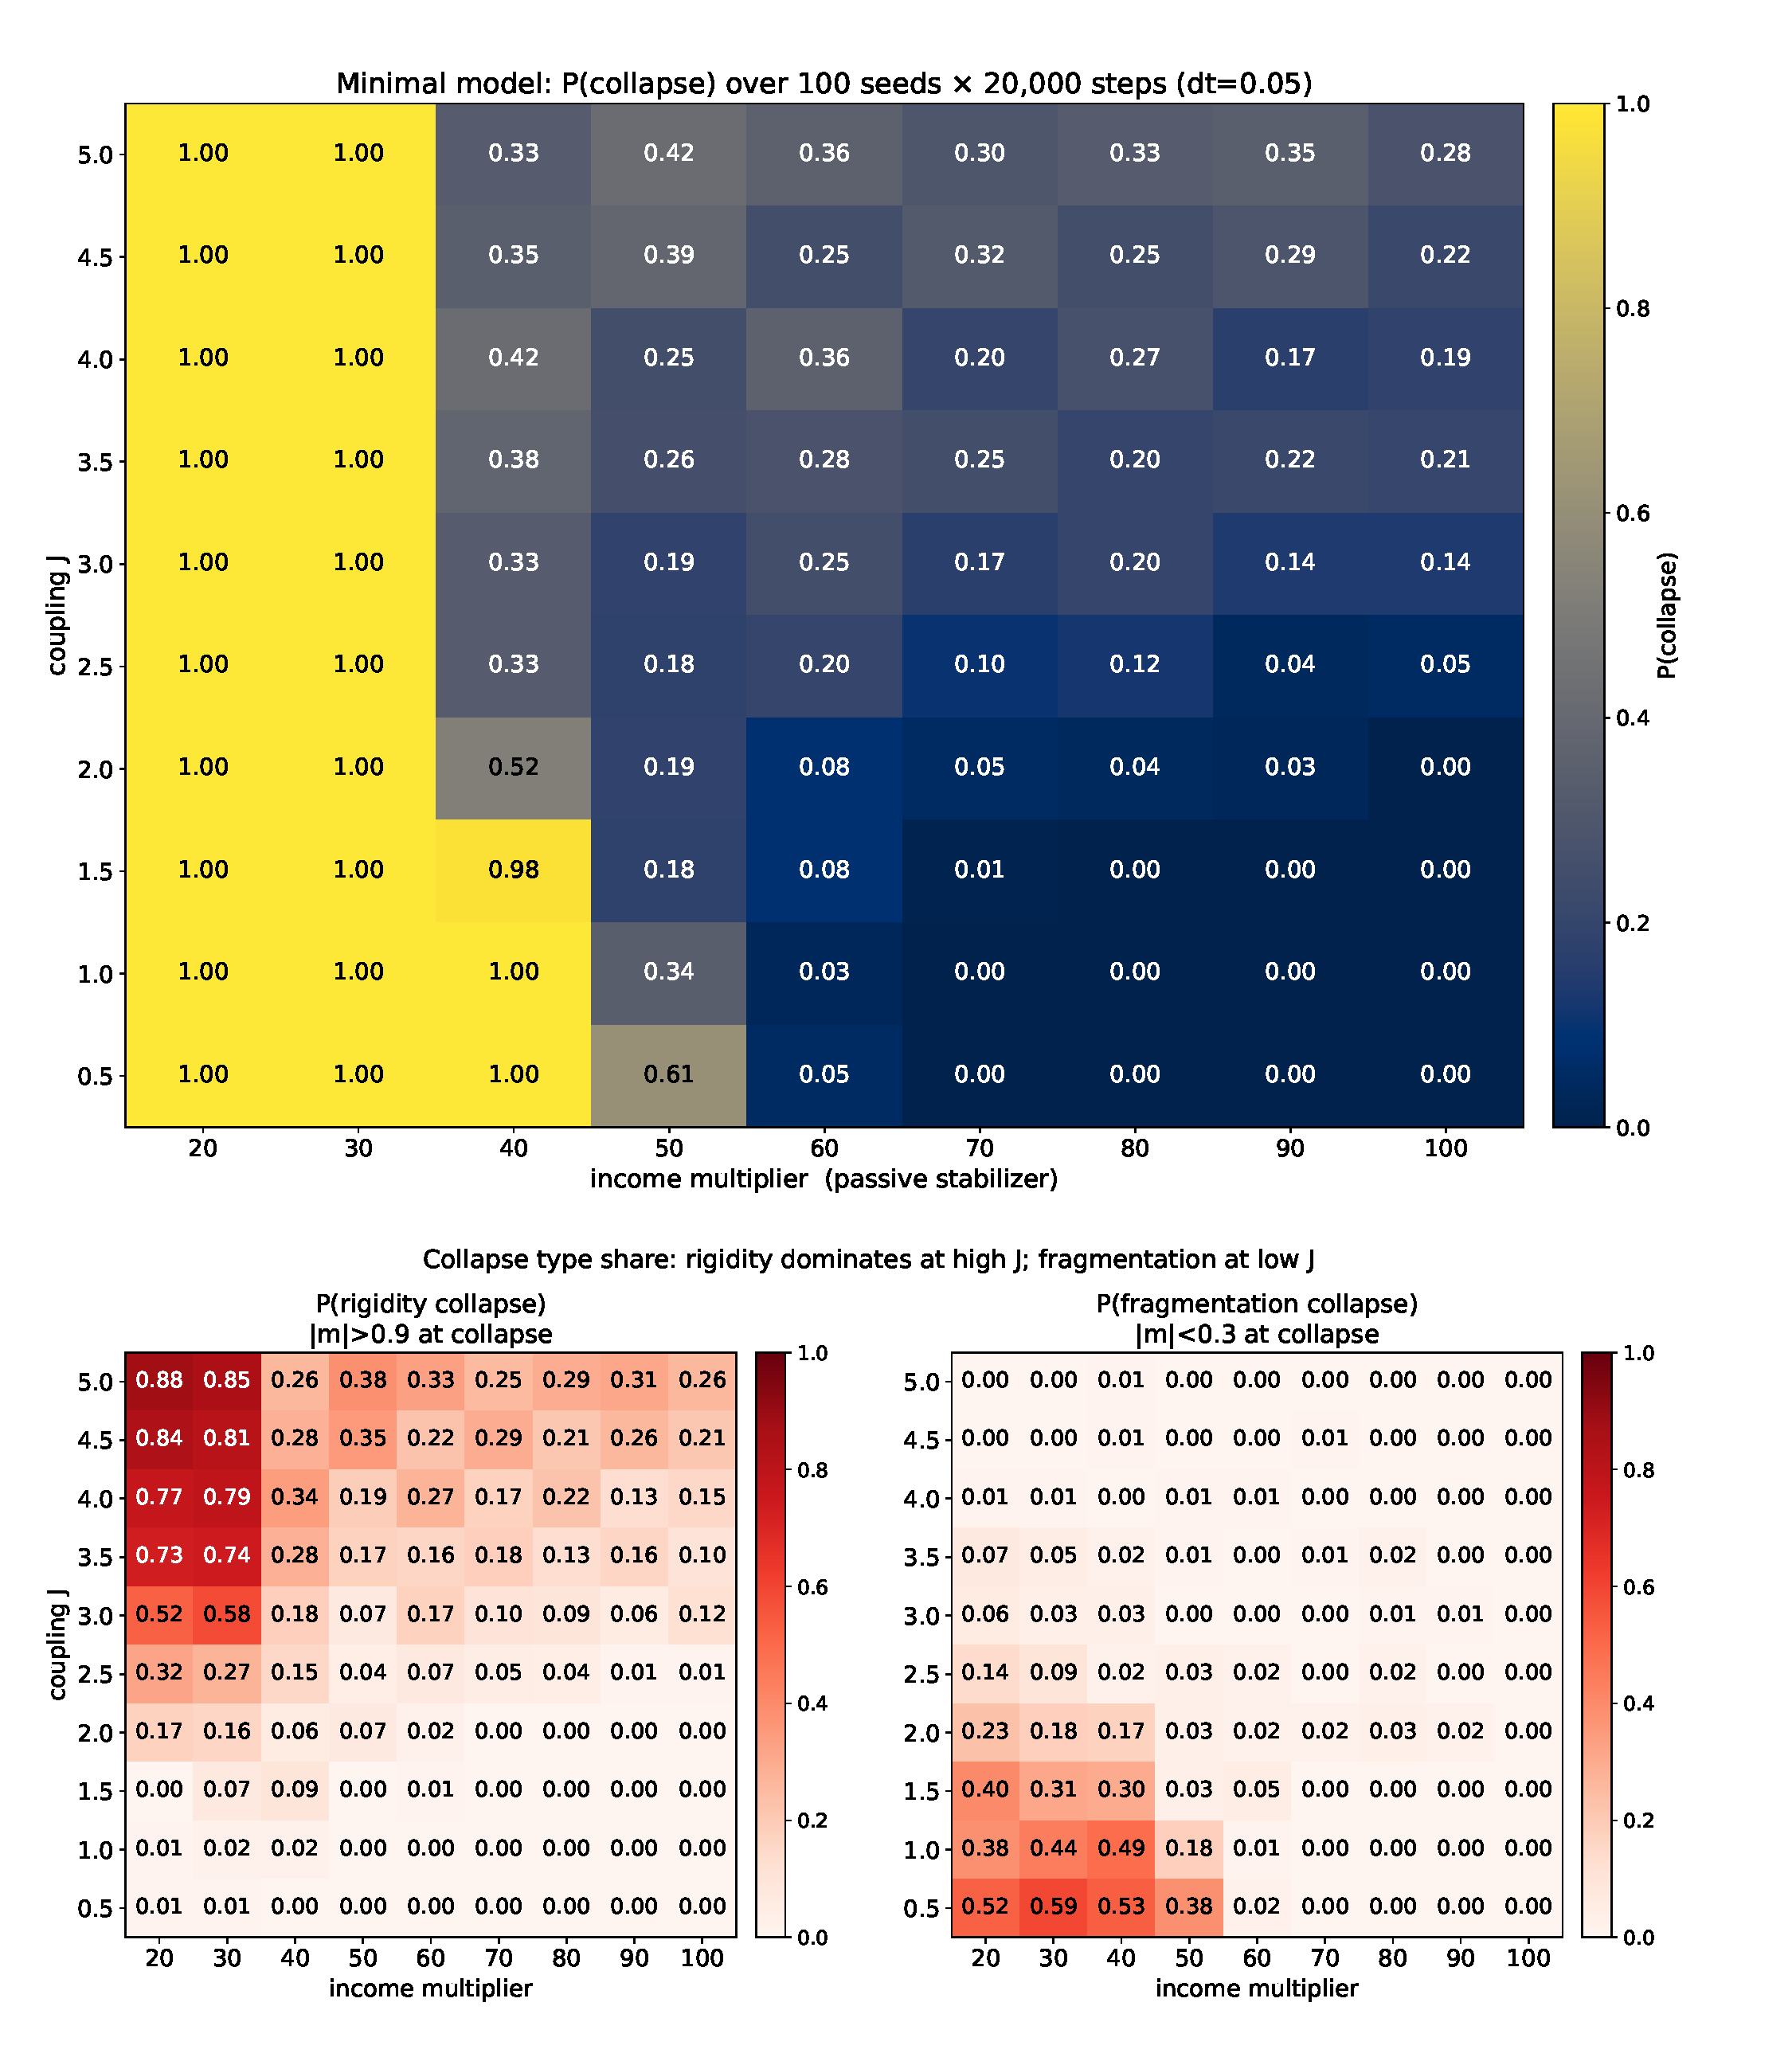
\includegraphics[width=0.95\textwidth]{figures/fig1.pdf}
\caption{\textit{Static asymmetry in the minimal model.} P(collapse) over the (\emph{J}, \emph{μ}) grid with per-cell P(rigidity collapse) and P(fragmentation collapse). 9,000 runs at d\emph{t} = 0.05, 100 seeds/cell. Fragmentation fills the low-\emph{J}, low-\emph{μ} corner (cured by raising \emph{μ}); rigidity dominates the high-\emph{J} band at every \emph{μ}, with a residual P(collapse) = 0.23 at \emph{μ} = 100 (90\% of collapsed runs rigidity-typed across the \emph{J} ≥ 4.0, \emph{μ} = 100 band, clipped-EM \textbar{}\emph{m}\textbar{} = 0.9 gate; type shares carry the integrator-scheme caveat of Supplementary Section S4).}
\label{fig:fig1}
\end{figure*}



\begin{figure*}[!htbp]
\centering
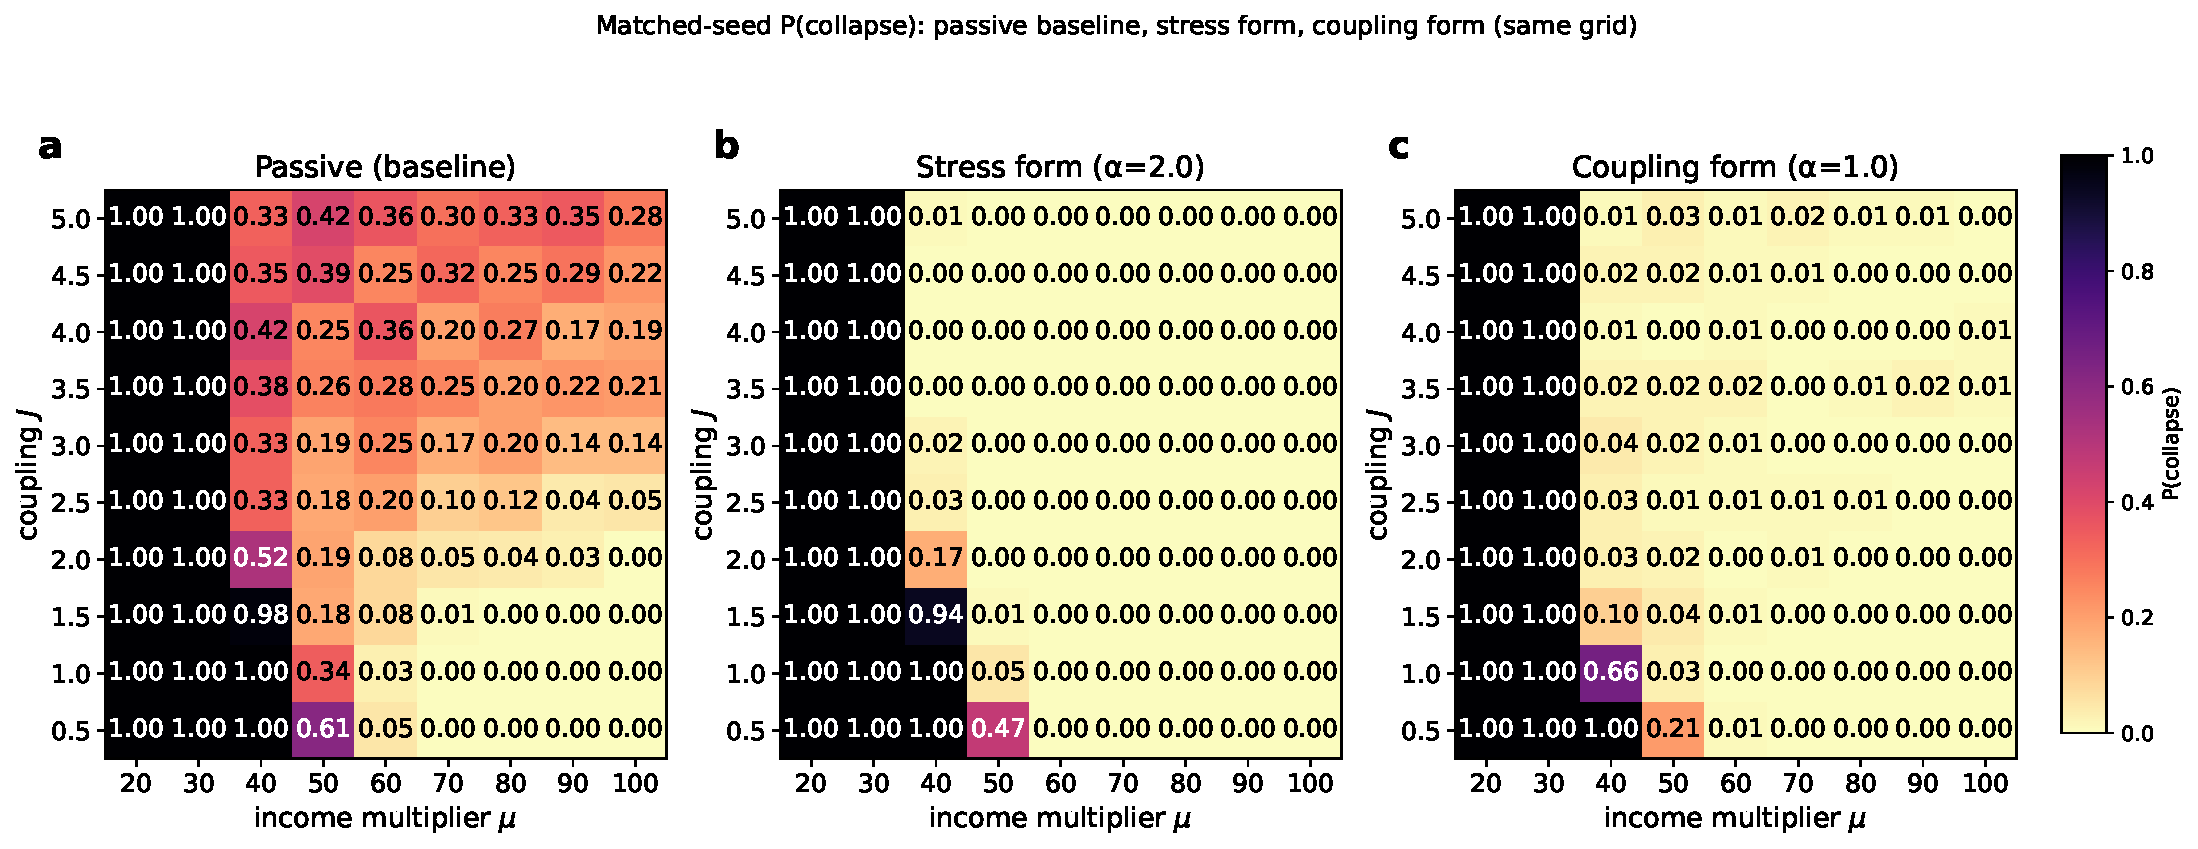
\includegraphics[width=0.95\textwidth]{figures/fig2.pdf}
\caption{\textit{Matched-seed stabilizer contrast.} Matched-seed P(collapse) over (\emph{J}, \emph{μ}): wealth-fed baseline \emph{h} = 2·(\emph{W}/500) (a, left), stress form (α = 2.0, b, center), coupling form (α = 1.0, c, right). The baseline reproduces the high-\emph{J} residual (band-mean 0.23 at \emph{μ} = 100); the stress and coupling forms show P(collapse) = 0.00 across \emph{J} ≥ 4.0 at \emph{μ} = 100 (95\% upper bound 0.03 per 100-seed cell) and ≤ 0.01 respectively. 9,000 runs/condition, d\emph{t} = 0.05. The contrast stands as a measurement. A pre-registered magnitude-matched control (E2; Results; Supplementary Section S5.6) shows that matching a stabilizer's full-trajectory delivered mean does not reproduce its outcome: a pure constant carrying the stress form's full-trajectory delivered mean collapses far less than the stress form at an informative operating point (0.000 vs 0.281, REFUTED in all three cells). The contrast is reported here as a measurement, not as evidence for a single delivered-amplitude cause.}
\label{fig:fig2}
\end{figure*}



\begin{figure*}[!htbp]
\centering
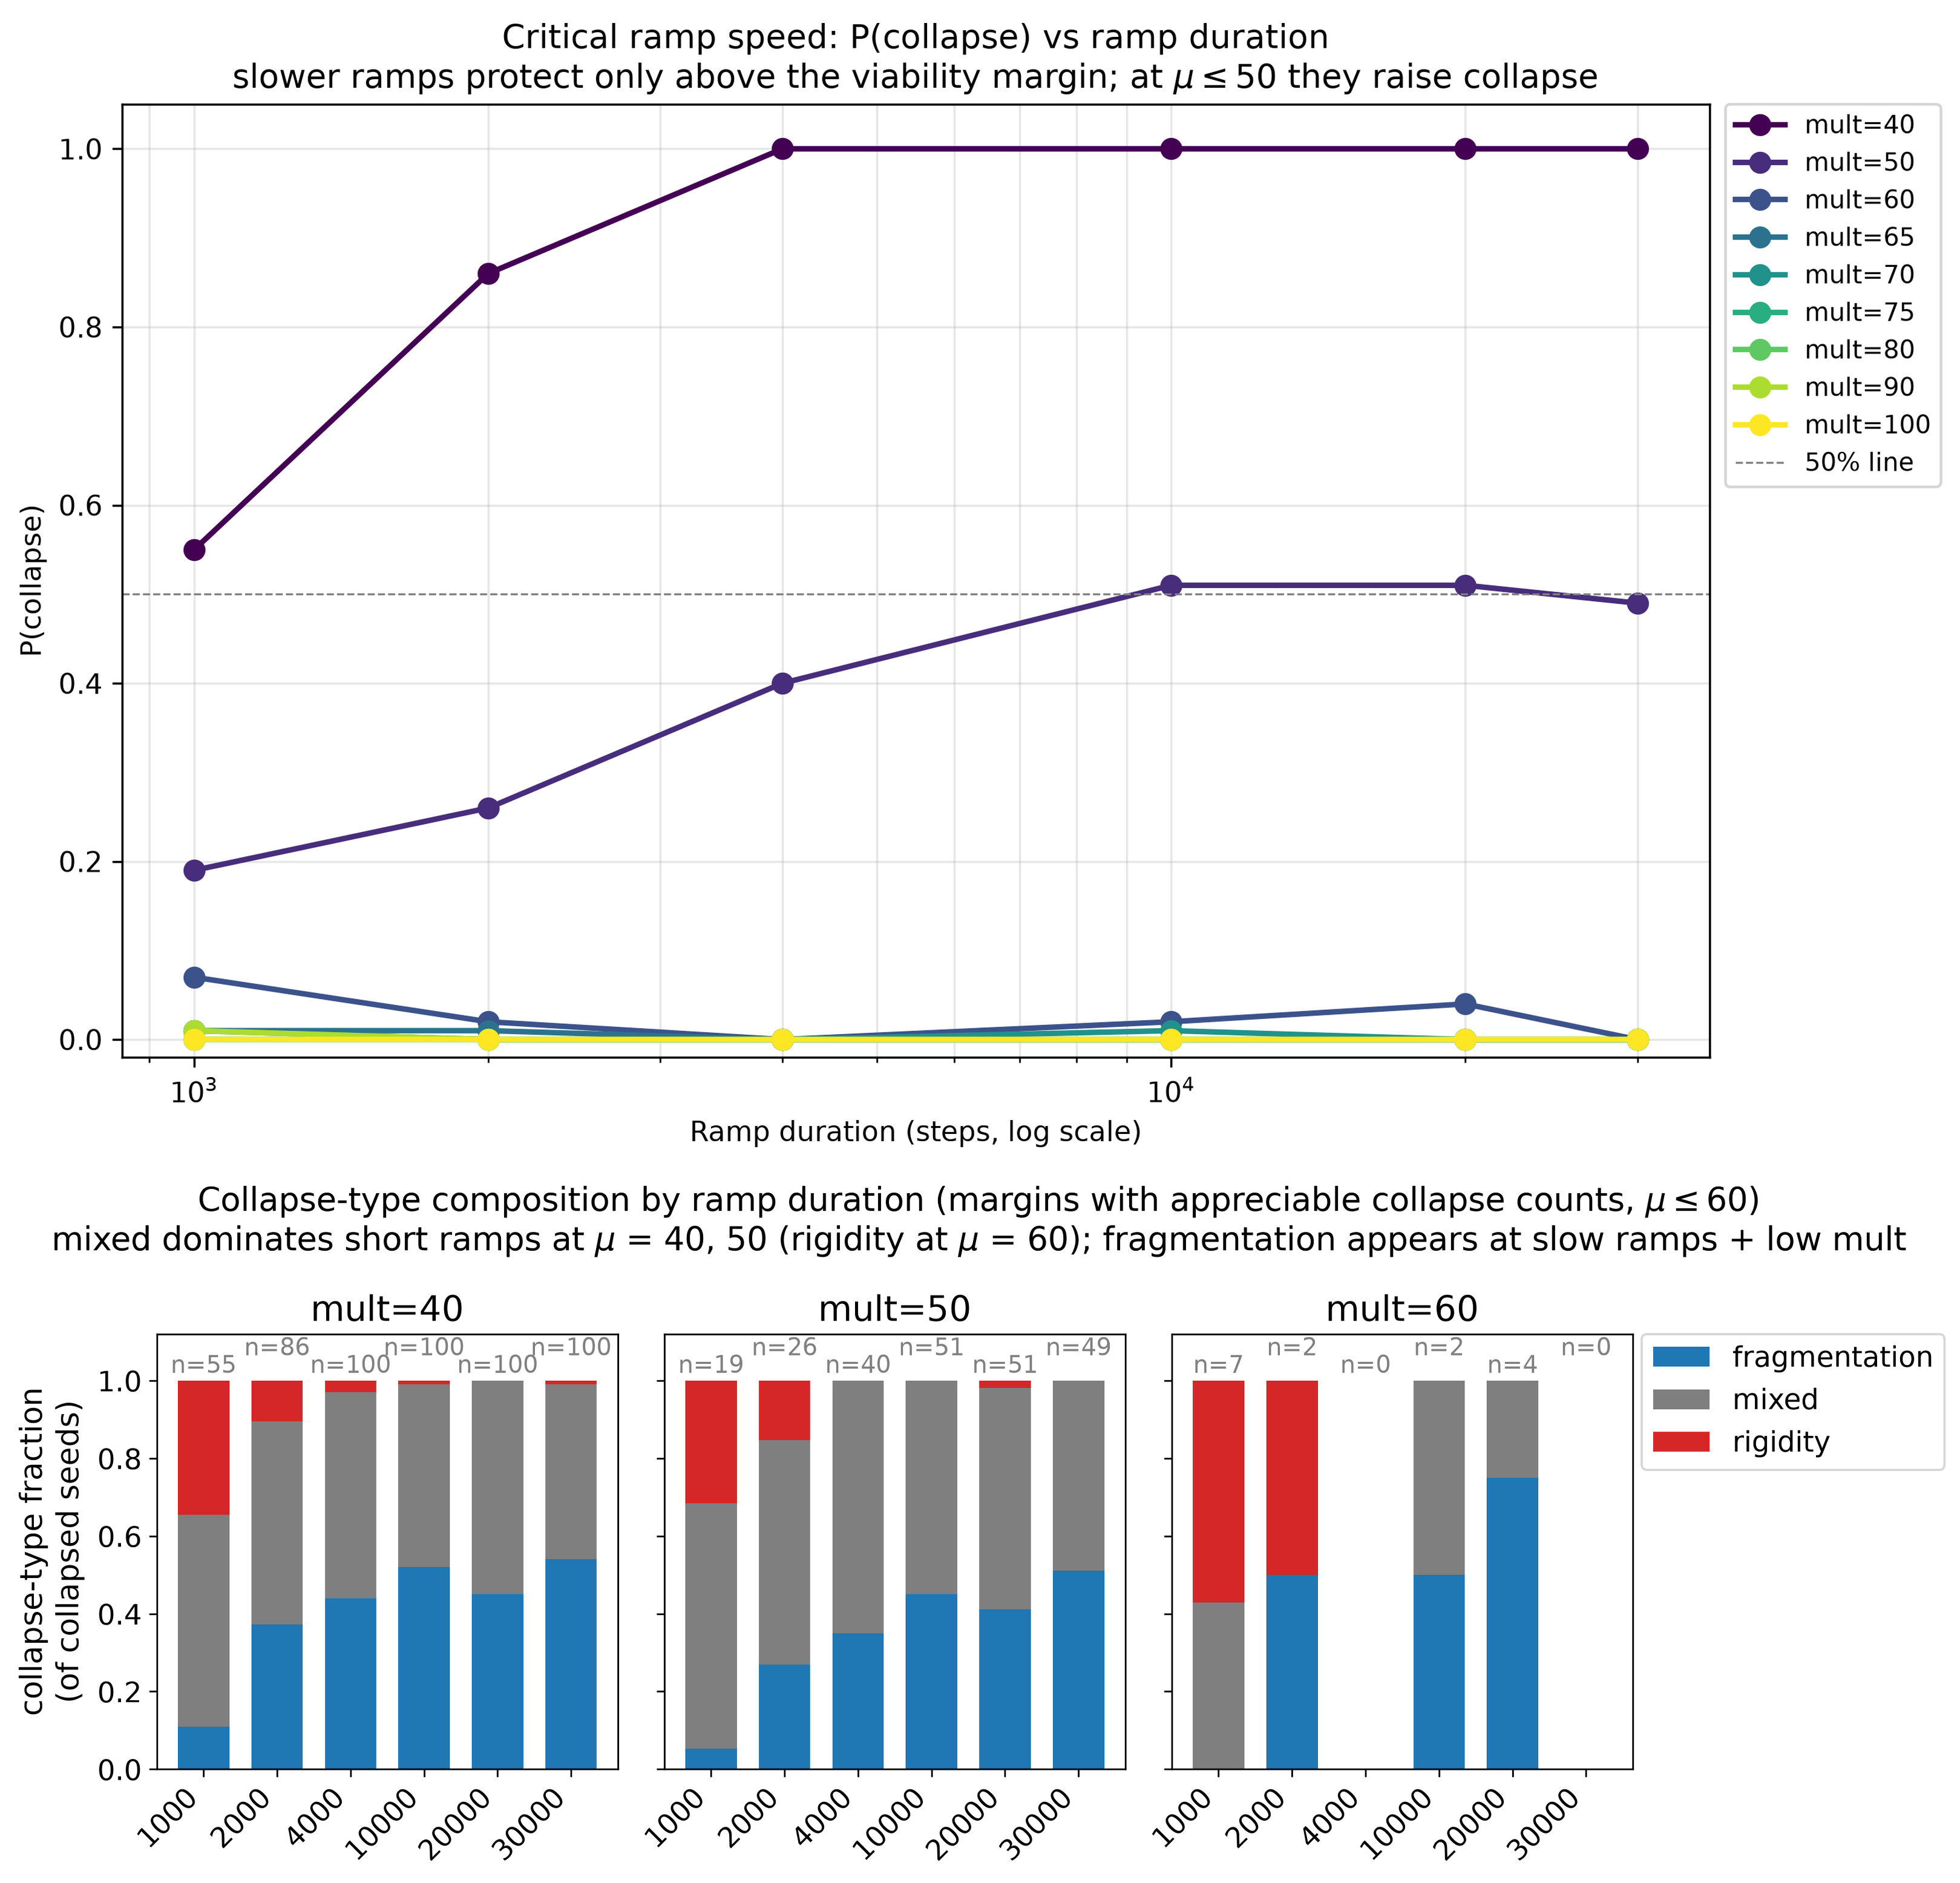
\includegraphics[width=0.95\textwidth]{figures/fig3.pdf}
\caption{\textit{Critical ramp speed.} P(collapse) vs ramp duration by margin \emph{μ}, with collapse-type composition (lower row shown for the margins with appreciable collapse counts, \emph{μ} ≤ 60; \emph{μ} ≥ 65 have ≤ 1 collapsed seed). Three regimes: resilient (\emph{μ} ≥ 60, ≤ 0.07), critical (\emph{μ} = 50, 0.50 near 9,200 steps), unviable (\emph{μ} = 40, the lowest margin swept: saturated at 1.00 beyond ramp ≈4,000 steps). At low margins the rigidity share collapses to ≈0 under slow ramps (clipped-EM \textbar{}\emph{m}\textbar{} = 0.9 gate; scheme caveat, Supplementary Section S4) and fragmentation becomes the largest typed class. 5,400 runs, d\emph{t} = 0.05; 100 seeds per point, so binomial 95\% CIs have half-width ≤ ±0.10 (≈±0.10 at P ≈ 0.5, ≈±0.05 at P ≈ 0.07).}
\label{fig:fig3}
\end{figure*}



\begin{figure*}[!htbp]
\centering
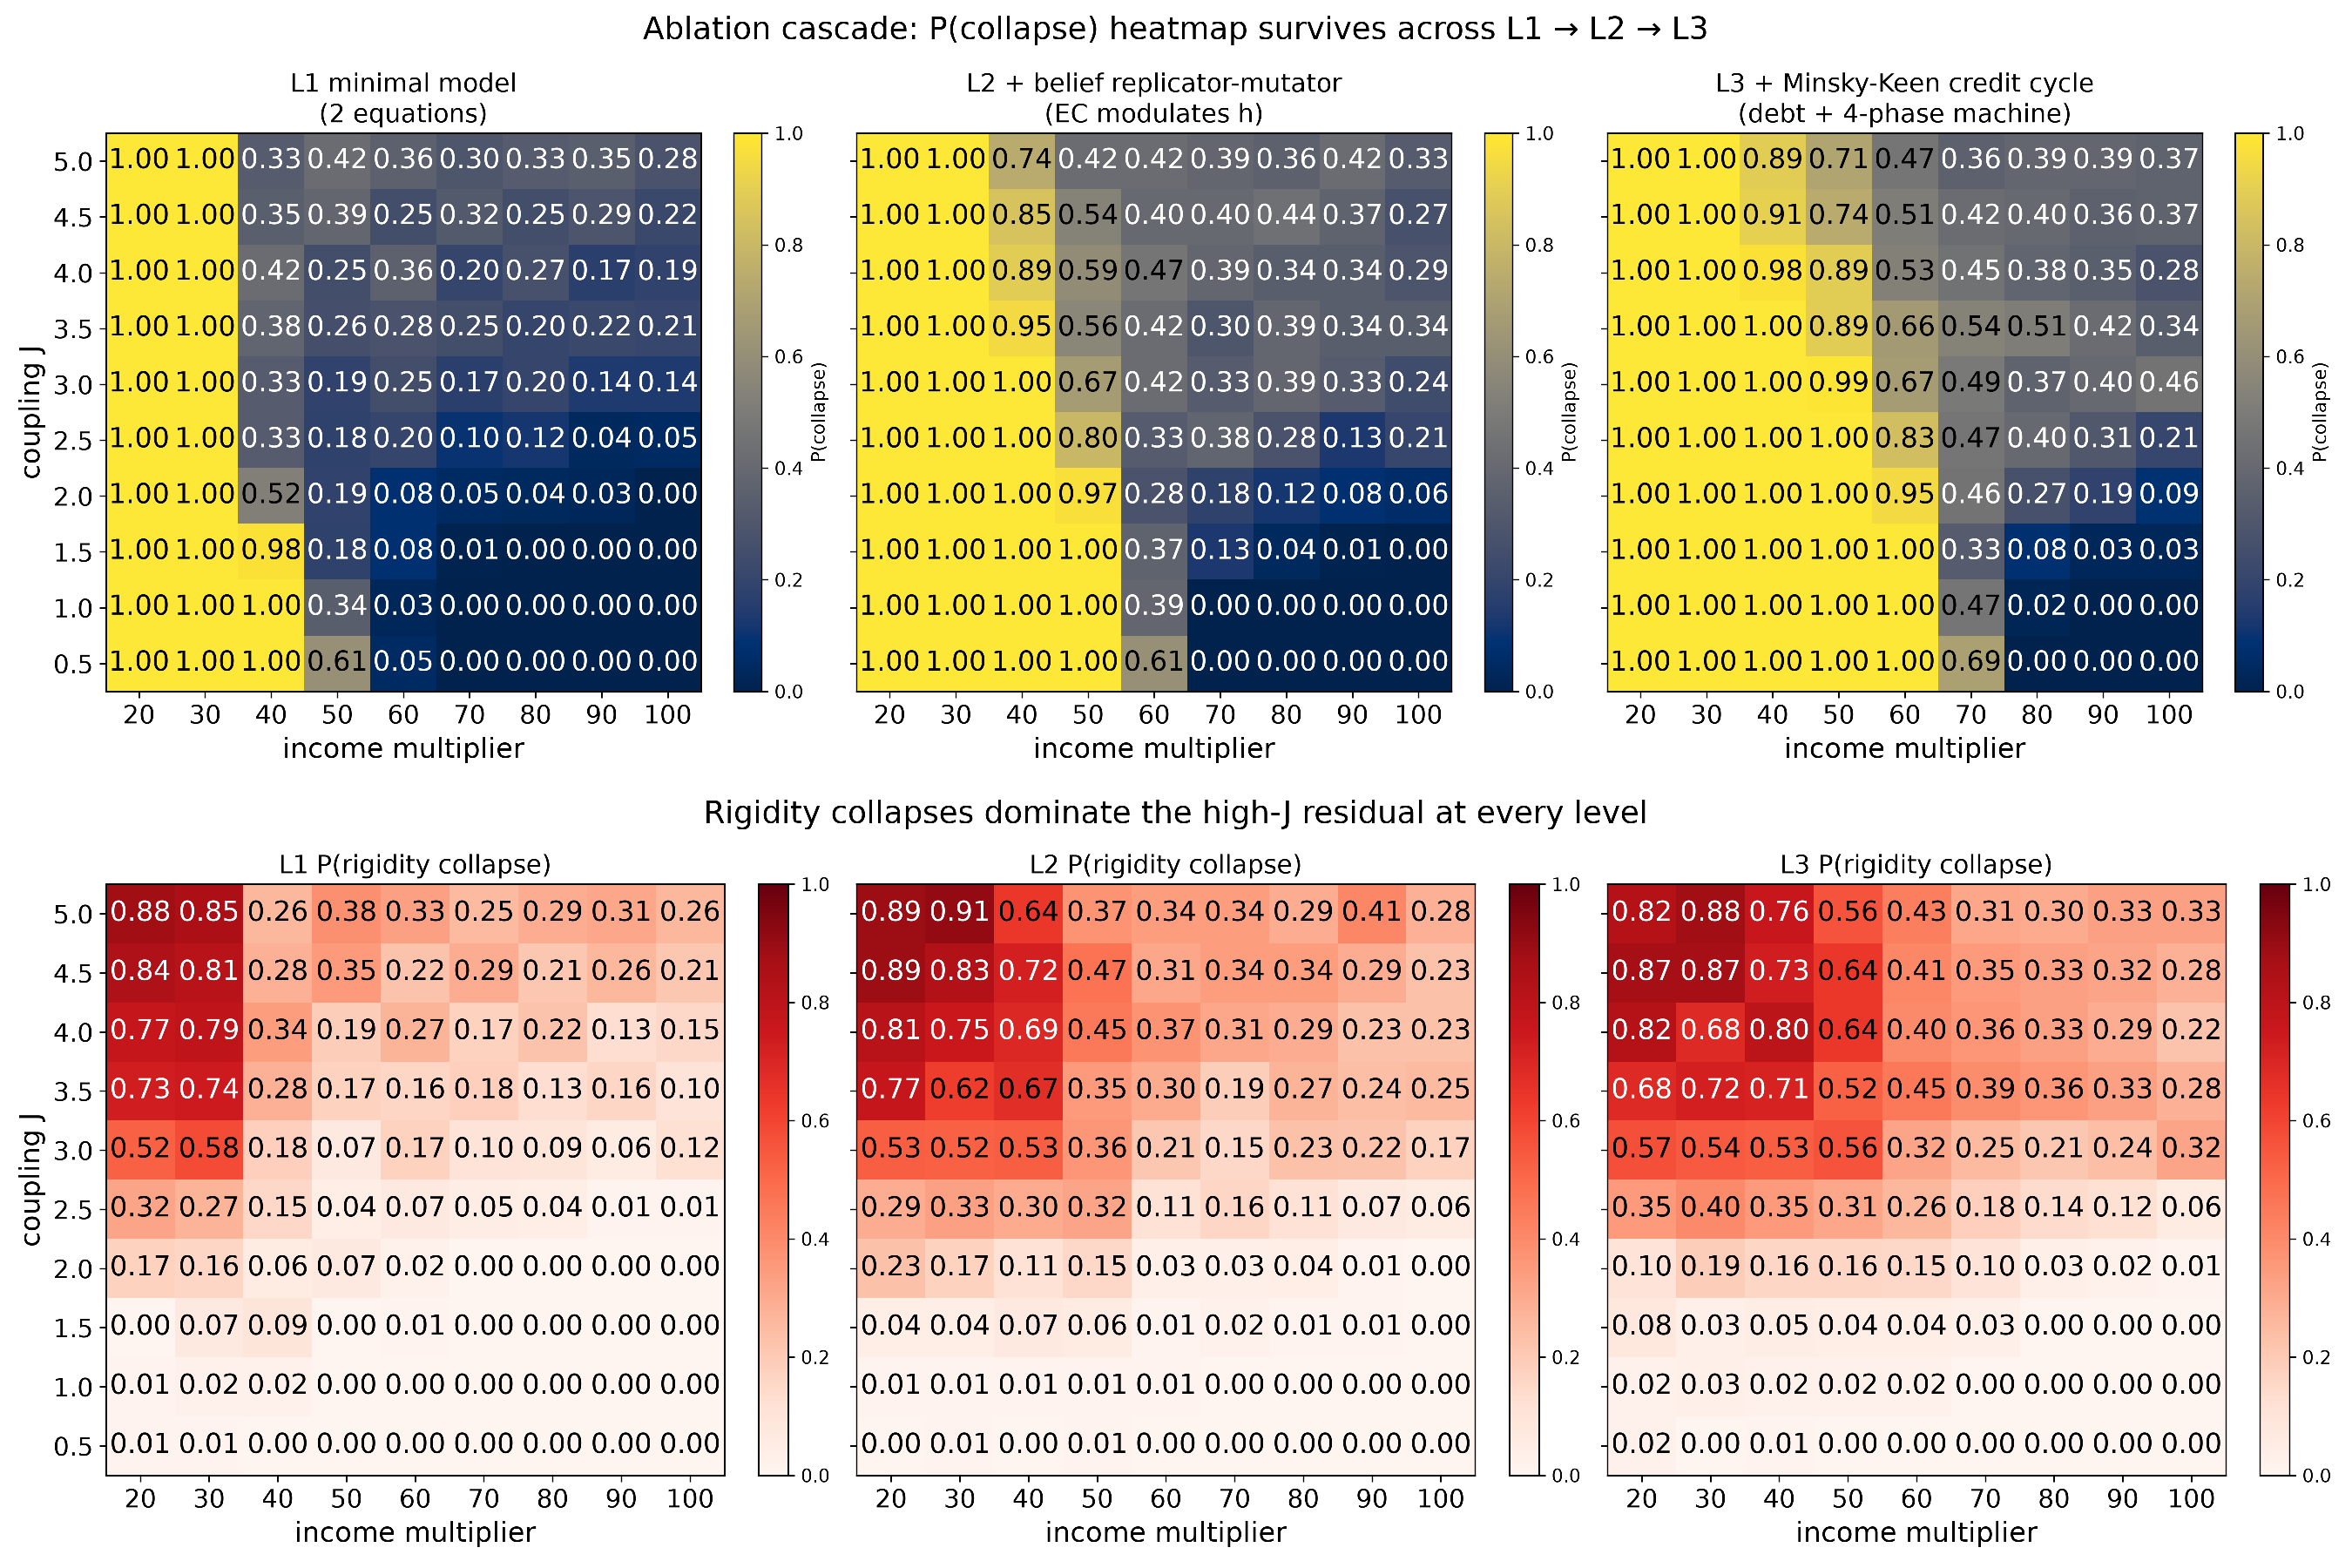
\includegraphics[width=0.95\textwidth]{figures/fig4.pdf}
\caption{\textit{Ablation cascade L1 → L2 → L3.} P(collapse) and per-cell P(rigidity collapse) heatmaps on the same (\emph{J}, \emph{μ}) grid as Figure 1. Adding belief (L2) and credit-cycle (L3) dynamics raises the high-\emph{J} residual point estimates (23\% → 30\% → 34\% at \emph{μ} = 100; the levels use independent seed bases, so the comparison is unpaired --- L1 → L3 +0.11, 95\% CI {[}+0.04, +0.18{]}, adjacent steps within sampling error) while rigidity remains the dominant type among collapsed runs (90\%, 83\%, 81\%, from the level summary CSVs; clipped-EM gate, Supplementary Section S4).}
\label{fig:fig4}
\end{figure*}



\begin{figure*}[!htbp]
\centering
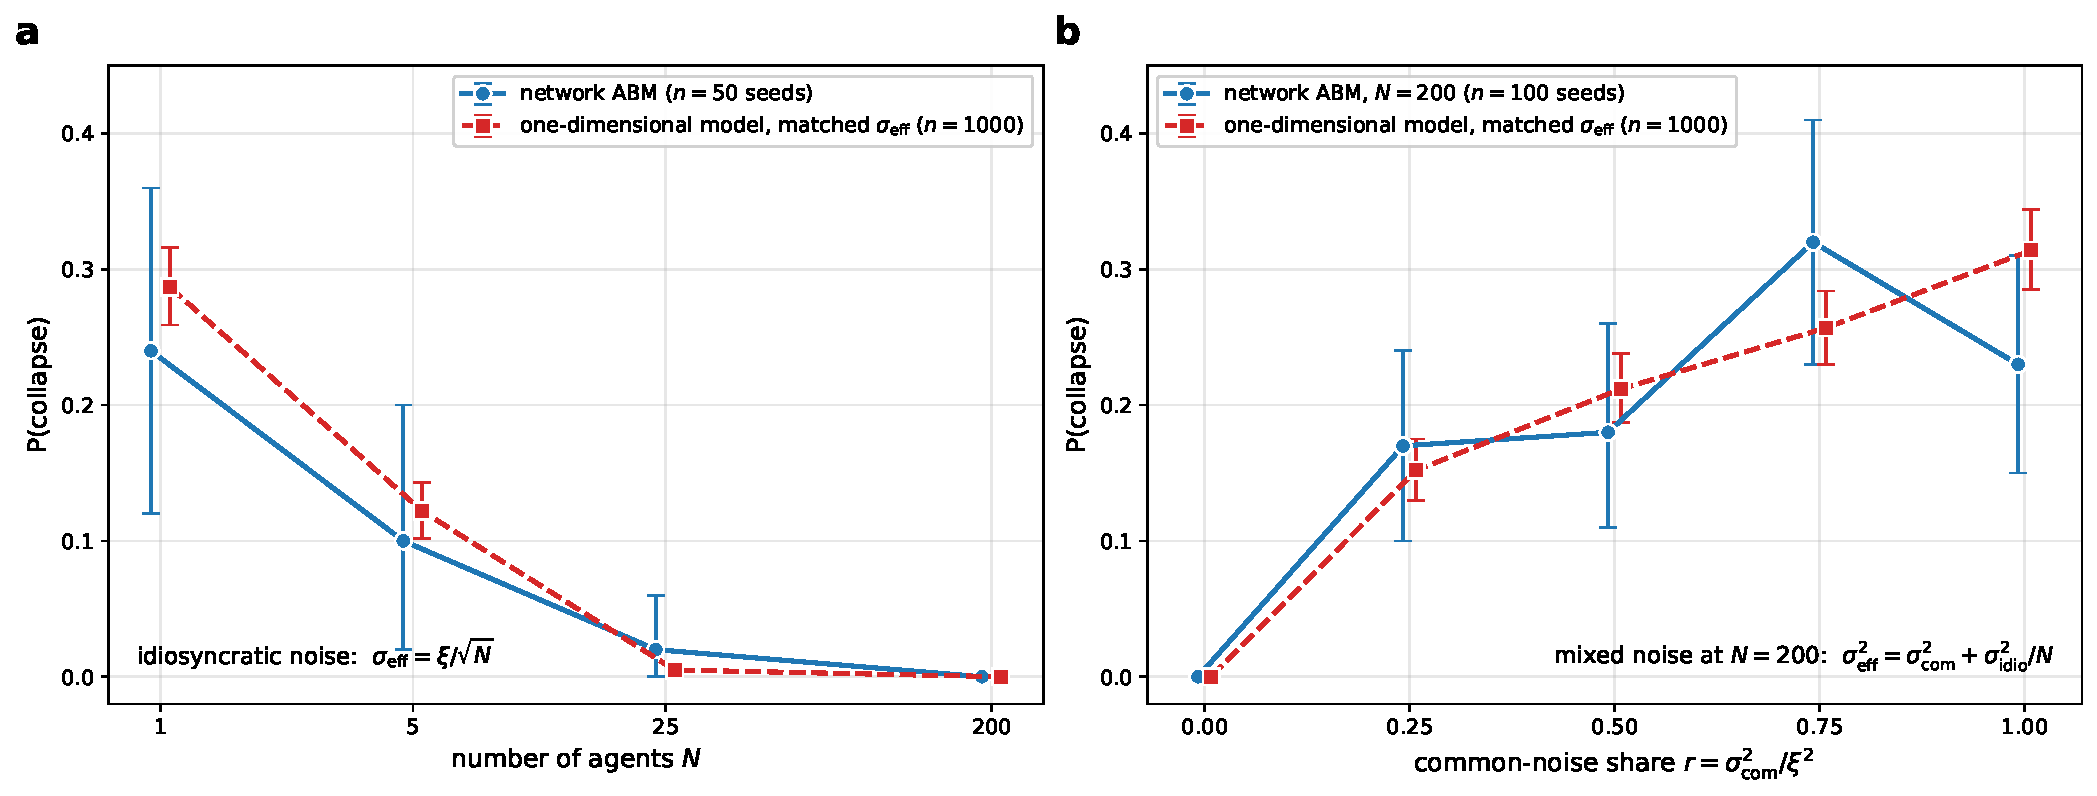
\includegraphics[width=0.95\textwidth]{figures/fig5.pdf}
\caption{\textit{Validity range of the one-dimensional reduction.} (a) Left: \emph{N}-scan at the idiosyncratic-noise endpoint --- ABM P(collapse) at \emph{N} ∈ \{1, 5, 25, 200\} (50 seeds/point) against the scalar model at the matched effective amplitude \(\sigma_{\mathrm{eff}}\) = \emph{ξ}/\(\sqrt{N}\) (\emph{ξ} = 0.5; \emph{n} = 1,000/point): 0.24/0.10/0.02/0.00 (ABM) vs 0.287/0.122/0.005/0.000 (scalar). (b) Right: mixed-noise sweep at \emph{N} = 200 --- common-mode share \emph{r} ∈ \{0, 0.25, 0.5, 0.75, 1.0\} of a fixed total noise budget, ABM (\emph{n} = 100/point) vs scalar at matched \(\sigma_{\mathrm{eff}}^2\) = \(\sigma_{\mathrm{com}}^2\) + \(\sigma_{\mathrm{idio}}^2\)/\emph{N}: 0.00/0.17/0.18/0.32/0.23 vs 0.000/0.152/0.212/0.257/0.314. The scalar reduction reproduces the ABM collapse statistics within binomial sampling error (ABM SE ≈ 0.02--0.06; largest gap 0.23 vs 0.314 at \emph{r} = 1.00, ≈2 SE) across the tested noise compositions; because \(\sigma_{\mathrm{eff}}\) is an identity, the agreement documents the validity range of the reduction used throughout --- no network or \emph{N} effect is claimed (\emph{J} = 5, \emph{μ} = 100; Supplementary Section S6).}
\label{fig:fig5}
\end{figure*}



\end{document}
